% ****** Start of file apssamp.tex ******
%
%   This file is part of the APS files in the REVTeX 4.1 distribution.
%   Version 4.1r of REVTeX, August 2010
%
%   Copyright (c) 2009, 2010 The American Physical Society.
%
%   See the REVTeX 4 README file for restrictions and more information.
%
% TeX'ing this file requires that you have AMS-LaTeX 2.0 installed
% as well as the rest of the prerequisites for REVTeX 4.1
%
% See the REVTeX 4 README file
% It also requires running BibTeX. The commands are as follows:
%
%  1)  latex apssamp.tex
%  2)  bibtex apssamp
%  3)  latex apssamp.tex
%  4)  latex apssamp.tex
%
\documentclass[%
aps, prd, reprint, show pacs, preprint numbers, ams math, amssymb, superscriptaddress, linenumbers]{revtex4-1}

\usepackage{amssymb,amsmath,amstext,nicefrac}
\usepackage{graphicx}% Include figure files
\usepackage{dcolumn}% Align table columns on decimal point
\usepackage{bm}% bold math
\usepackage{xspace}
\usepackage{xcolor}
\usepackage[tight]{subfigure}
\usepackage{longtable}
\usepackage{lineno}
\usepackage{pstricks}
\usepackage{appendix}
\usepackage{units}

%\def\dedx{$\langle dE/dx\rangle$\xspace}
\newcommand{\dedx}{\ensuremath{\langle dE/dx\rangle}\xspace}
\def\pzpt{$(p_\mathrm{z},p_\mathrm{T})$\xspace}

\makeatother
\linenumbers

\begin{document}

\preprint{FERMILAB-PUB-XX-XXX-E, hep-ex YYYY.ZZZZ}

\title{Measurement of Pion Production Yields off the NuMI Target}% Force line breaks with \\
%\thanks{A footnote to the article title}%

%Collaboration list
\newcommand{\FNAL}{Fermi National Accelerator Laboratory, Batavia, Illinois 60510, USA}
\newcommand{\ANL}{Argonne National Laboratory, Argonne, Illinois 60439, USA}
\newcommand{\Indiana}{Indiana University, Bloomington, Indiana 47403, USA}
\newcommand{\Harvard}{Department of Physics, Harvard University, Cambridge, Massachusetts 02138, USA}
\newcommand{\LLNL}{Lawrence Livermore National Laboratory, Livermore, California 94550, USA}
\newcommand{\USC}{Department of Physics and Astronomy, University of South Carolina, Columbia, South Carolina 29208, USA}
\newcommand{\Iowa}{University of Iowa, COE College, Cedar Rapids, Iowa, USA}
\newcommand{\UVa}{University of Virginia, Charlotteville, Virginia, USA}
\newcommand{\ELM}{Elmhurst College, Elmhurst, Ilinois, USA}
\newcommand{\IIT}{Illinois Institute of Technology, Chicago, Illinois 60616 USA}
\newcommand{\Purdue}{Purdue University, Lafeyette, Indiana, USA}
\newcommand{\UCB}{University of Colorado, Boulder, Colorado, USA}
\newcommand{\UM}{University of Michigan, Ann Arbor, Michigan, USA}
\newcommand{\MI}{Muons, Inc., Batavia, Illinois, USA}
\newcommand{\Wichita}{Wichita State University, Wichita, Kansas, USA}
\newcommand{\Delhi}{University of Delhi, Delhi 110007, India}
\newcommand{\Panjab}{Panjab University, Chandigarh 160014, India}
\newcommand{\deceased}{Deceased.}
\newcommand{\COE}{COE College, Cedar Rapids, Iowa, USA}
\newcommand{\Sutcu}{Now at Kahramanmaras Sutcu Imam University, Kahramanmaras, Turkey}
\newcommand{\CalPoly}{Now at California Polytechnical State University}
\newcommand{\Queens}{Now at Queen's University, Canada}
\newcommand{\Mustafa}{Now at Mustafa Kemal University, Hatay, Turkey}
\newcommand{\PNNL}{Now at Pacific Northwest National Laboratory, Richland, WA 99352, USA}
\newcommand{\FNALNow}{Now at Fermi National Accelerator Laboratory}
\newcommand{\Pitt}{Now at University of Pittsburgh, Pittsburgh, Pennsylvania, USA}
\newcommand{\BOG}{Now at Bogazici University, Istanbul, Turkey}

\affiliation{\ANL}
\affiliation{\COE}
\affiliation{\UCB}
\affiliation{\Delhi}
\affiliation{\ELM}
\affiliation{\FNAL}
\affiliation{\Harvard}
\affiliation{\IIT}
\affiliation{\Indiana}
\affiliation{\Iowa}
\affiliation{\LLNL}
\affiliation{\UM}
\affiliation{\MI}
\affiliation{\Panjab}
\affiliation{\Purdue}
\affiliation{\USC}
\affiliation{\UVa}
\affiliation{\Wichita}
\affiliation{\BOG}
\affiliation{\CalPoly}
\affiliation{\FNALNow}
\affiliation{\Mustafa}
\affiliation{\PNNL}
\affiliation{\Pitt}
\affiliation{\Queens}
\affiliation{\Sutcu}

\author{Jonathan M. Paley}
\affiliation{\ANL}

\author{M.D.~Messier}
\affiliation{\Indiana}

\author{R.~Raja}
\affiliation{\FNAL}
\affiliation{\deceased}

\author{R.~J.~Abrams}
\affiliation{\UM}
\affiliation{\MI}

\author{U.~Akgun}
\affiliation{\Iowa}
\affiliation{\COE}

\author{D.~M.~Asner}
\affiliation{\LLNL}
\affiliation{\PNNL}

\author{G.~Aydin}
\affiliation{\Iowa}
\affiliation{\Mustafa}

\author{W.~Baker}
\affiliation{\FNAL}

\author{P.~D.~Barnes, Jr.~}
\affiliation{\LLNL}

\author{T.~Bergfeld}
\affiliation{\USC}

\author{L.~Beverly}
\affiliation{\FNAL}

\author{V.~Blatnagar}
\affiliation{\Panjab}

%\author{D.~Carey}
%\affiliation{\FNAL}

\author{B.~Choudhary}
\affiliation{\Delhi}

\author{E.~C.~Dukes}
\affiliation{\UVa}

\author{F.~Duru}
\affiliation{\Iowa}

\author{G.J.~Feldman}
\affiliation{\Harvard}

\author{A.~Godley}
\affiliation{\USC}

\author{N.~Graf}
\affiliation{\Indiana}
\affiliation{\Pitt}

\author{J.~Gronberg}
\affiliation{\LLNL}

\author{E.~G\"{u}lmez}
\affiliation{\Iowa}
\affiliation{\BOG}

\author{Y.O.~G\"{u}nayd{\"i}n}
\affiliation{\Iowa}
\affiliation{\Sutcu}

\author{H.~R.~Gustafson}
\affiliation{\UM}

\author{E.~P.~Hartouni}
\affiliation{\LLNL}

\author{P.~Hanlet}
\affiliation{\IIT}

%\author{S.~Hansen}
%\affiliation{\FNAL}

\author{M.~Heffner}
\affiliation{\LLNL}

%\author{C.~Johnstone}
%\affiliation{\FNAL}

\author{D.~M.~Kaplan}
\affiliation{\IIT}

\author{O.~Kamaev}
\affiliation{\IIT}
\affiliation{\Queens}

%\author{J.~Kilmer}
%\affiliation{\FNAL}

\author{J.~Klay}
\affiliation{\LLNL}
\affiliation{\CalPoly}

%\author{M.~Kostin}
%\affiliation{\FNAL}

\author{A.~Kumar}
\affiliation{\Panjab}

\author{D.~J.~Lange}
\affiliation{\LLNL}

\author{A.~Lebedev}
\affiliation{\Harvard}

\author{J.~Ling}
\affiliation{\USC}

\author{M.~Longo}
\affiliation{\UM}

\author{L.~C.~Lu}
\affiliation{\UVa}

\author{C.~Materniak}
\affiliation{\UVa}

\author{S.~Mahajan}
\affiliation{\Panjab}

\author{H.~Meyer}
\affiliation{\Wichita}

\author{D.~E.~Miller}
\affiliation{\Purdue}

\author{S.~R.~Mishra}
\affiliation{\USC}

\author{K.~Nelson}
\affiliation{\UVa}

\author{T.~Nigmanov}
\affiliation{\UM}
\affiliation{\Pitt}

\author{A.~Norman}
\affiliation{\UVa}
\affiliation{\FNALNow}

\author{Y.~Onel}
\affiliation{\Iowa}

\author{H.~K.~Park}
\affiliation{\UM}

\author{A.~Penzo}
\affiliation{\Iowa}

\author{R.~J.~Peterson}
\affiliation{\UCB}

\author{D.~Rajaram}
\affiliation{\IIT}

\author{D.~Ratnikov}
\affiliation{\IIT}

\author{C.~Rosenfeld}
\affiliation{\USC}

\author{H.~Rubin}
\affiliation{\IIT}

\author{S.~Seun}
\affiliation{\Harvard}

\author{A.~Singh}
\affiliation{\Panjab}

\author{N.~Solomey}
\affiliation{\Wichita}

\author{R.~A.~Soltz}
\affiliation{\LLNL}

%\author{E.~Swallow}
%\affiliation{\ELM}

%\author{R.~Schmitt}
%\affiliation{\FNAL}

\author{P.~Subbarao}
\affiliation{\UM}

\author{Y.~Torun}
\affiliation{\IIT}

%\author{T.~E.~Tope}
%\affiliation{\FNAL}

\author{K.~Wilson}
\affiliation{\USC}

\author{D.~M.~Wright}
\affiliation{\LLNL}

\author{Q.~K.~Wu}
\affiliation{\USC}

\collaboration{The MIPP Collaboration}
\noaffiliation

\date{\today}
\pacs{PACS 13.15.+g}

\begin{abstract}
The fixed-target Main Injector Particle Production (MIPP, Fermilab E907) Experiment was designed to measure the production of hadrons from the collisions of hadrons and mesons of momenta ranging from 5 to 120 GeV/c on nuclei.  These data will generally improve the simulation of particle detectors and predictions of particle beam  fluxes at accelerators.  The spectrometer momentum resolution is $< 5\%$, and particle identification is determined for particles 
ranging between 0.3 - 80 GeV/c using $dE/dx$, time-of-flight and Cherenkov radiation measurements.  MIPP 
collected $1.42 \times10^6$ events of 120 GeV Main Injector protons striking a target used in the Neutrinos at the Main Injector (NuMI) facility at Fermilab.  The NuMI target consists of 2 interaction lengths of graphite surrounded by a xx mm thick aluminum tube.  The data have been analyzed and we present here pion yields per proton-on-target determined in bins longitudinal and transverse momentum between 0.5 - 80 GeV/c, with $<10\%$ combined statistical and systematic relative uncertainties.

\end{abstract}

\pacs{Valid PACS appear here}% PACS, the Physics and Astronomy
                             % Classification Scheme.
%\keywords{Suggested keywords}%Use showkeys class option if keyword
                              %display desired
\maketitle

%\tableofcontents

\section{Introduction}
A growing number of neutrino experiments conducted at proton accelerators derive their neutrino beams from 
horn-focused beams of pions and kaons which result from proton-nucleus collisions in low-Z materials.  At the 
NuMI facility at Fermilab, hadron production uncertainties in Monte Carlo (MC) simulations generally dominate 
the uncertainties of the neutrino flux predictions at the level of 15-20\%, and are a limiting factor in the neutrino 
cross-section measurements being done by many NuMI-based experiments\cite{ref:MINOS},\cite{ref:MINERvA1},\cite{ref:MINERvA2}.  
Direct measurements of hadron production can be used to improve these MC simulations and reduce the 
uncertainties of the flux predictions.  One of the goals of the Main Injector Particle Production (MIPP) experiment 
was to measure the hadron production yield off of an actual NuMI target with 120 GeV/c protons from 
the Main Injector, which is the focus of this paper.  

%The Main Injector Particle Production (MIPP) Experiment at Fermi National 
%Accelerator Laboratory (FNAL) collected data in 2005 
%between 
%December 2004 and Februrary 2006 on a variety of fixed-target nuclei with a tertiary beam consisting of tagged 
%protons, charged pions and charged kaons over a momentum range from 5-120 GeV/c.  

\section{The MIPP Spectrometer}

\begin{figure}[tpb]
   \centering
   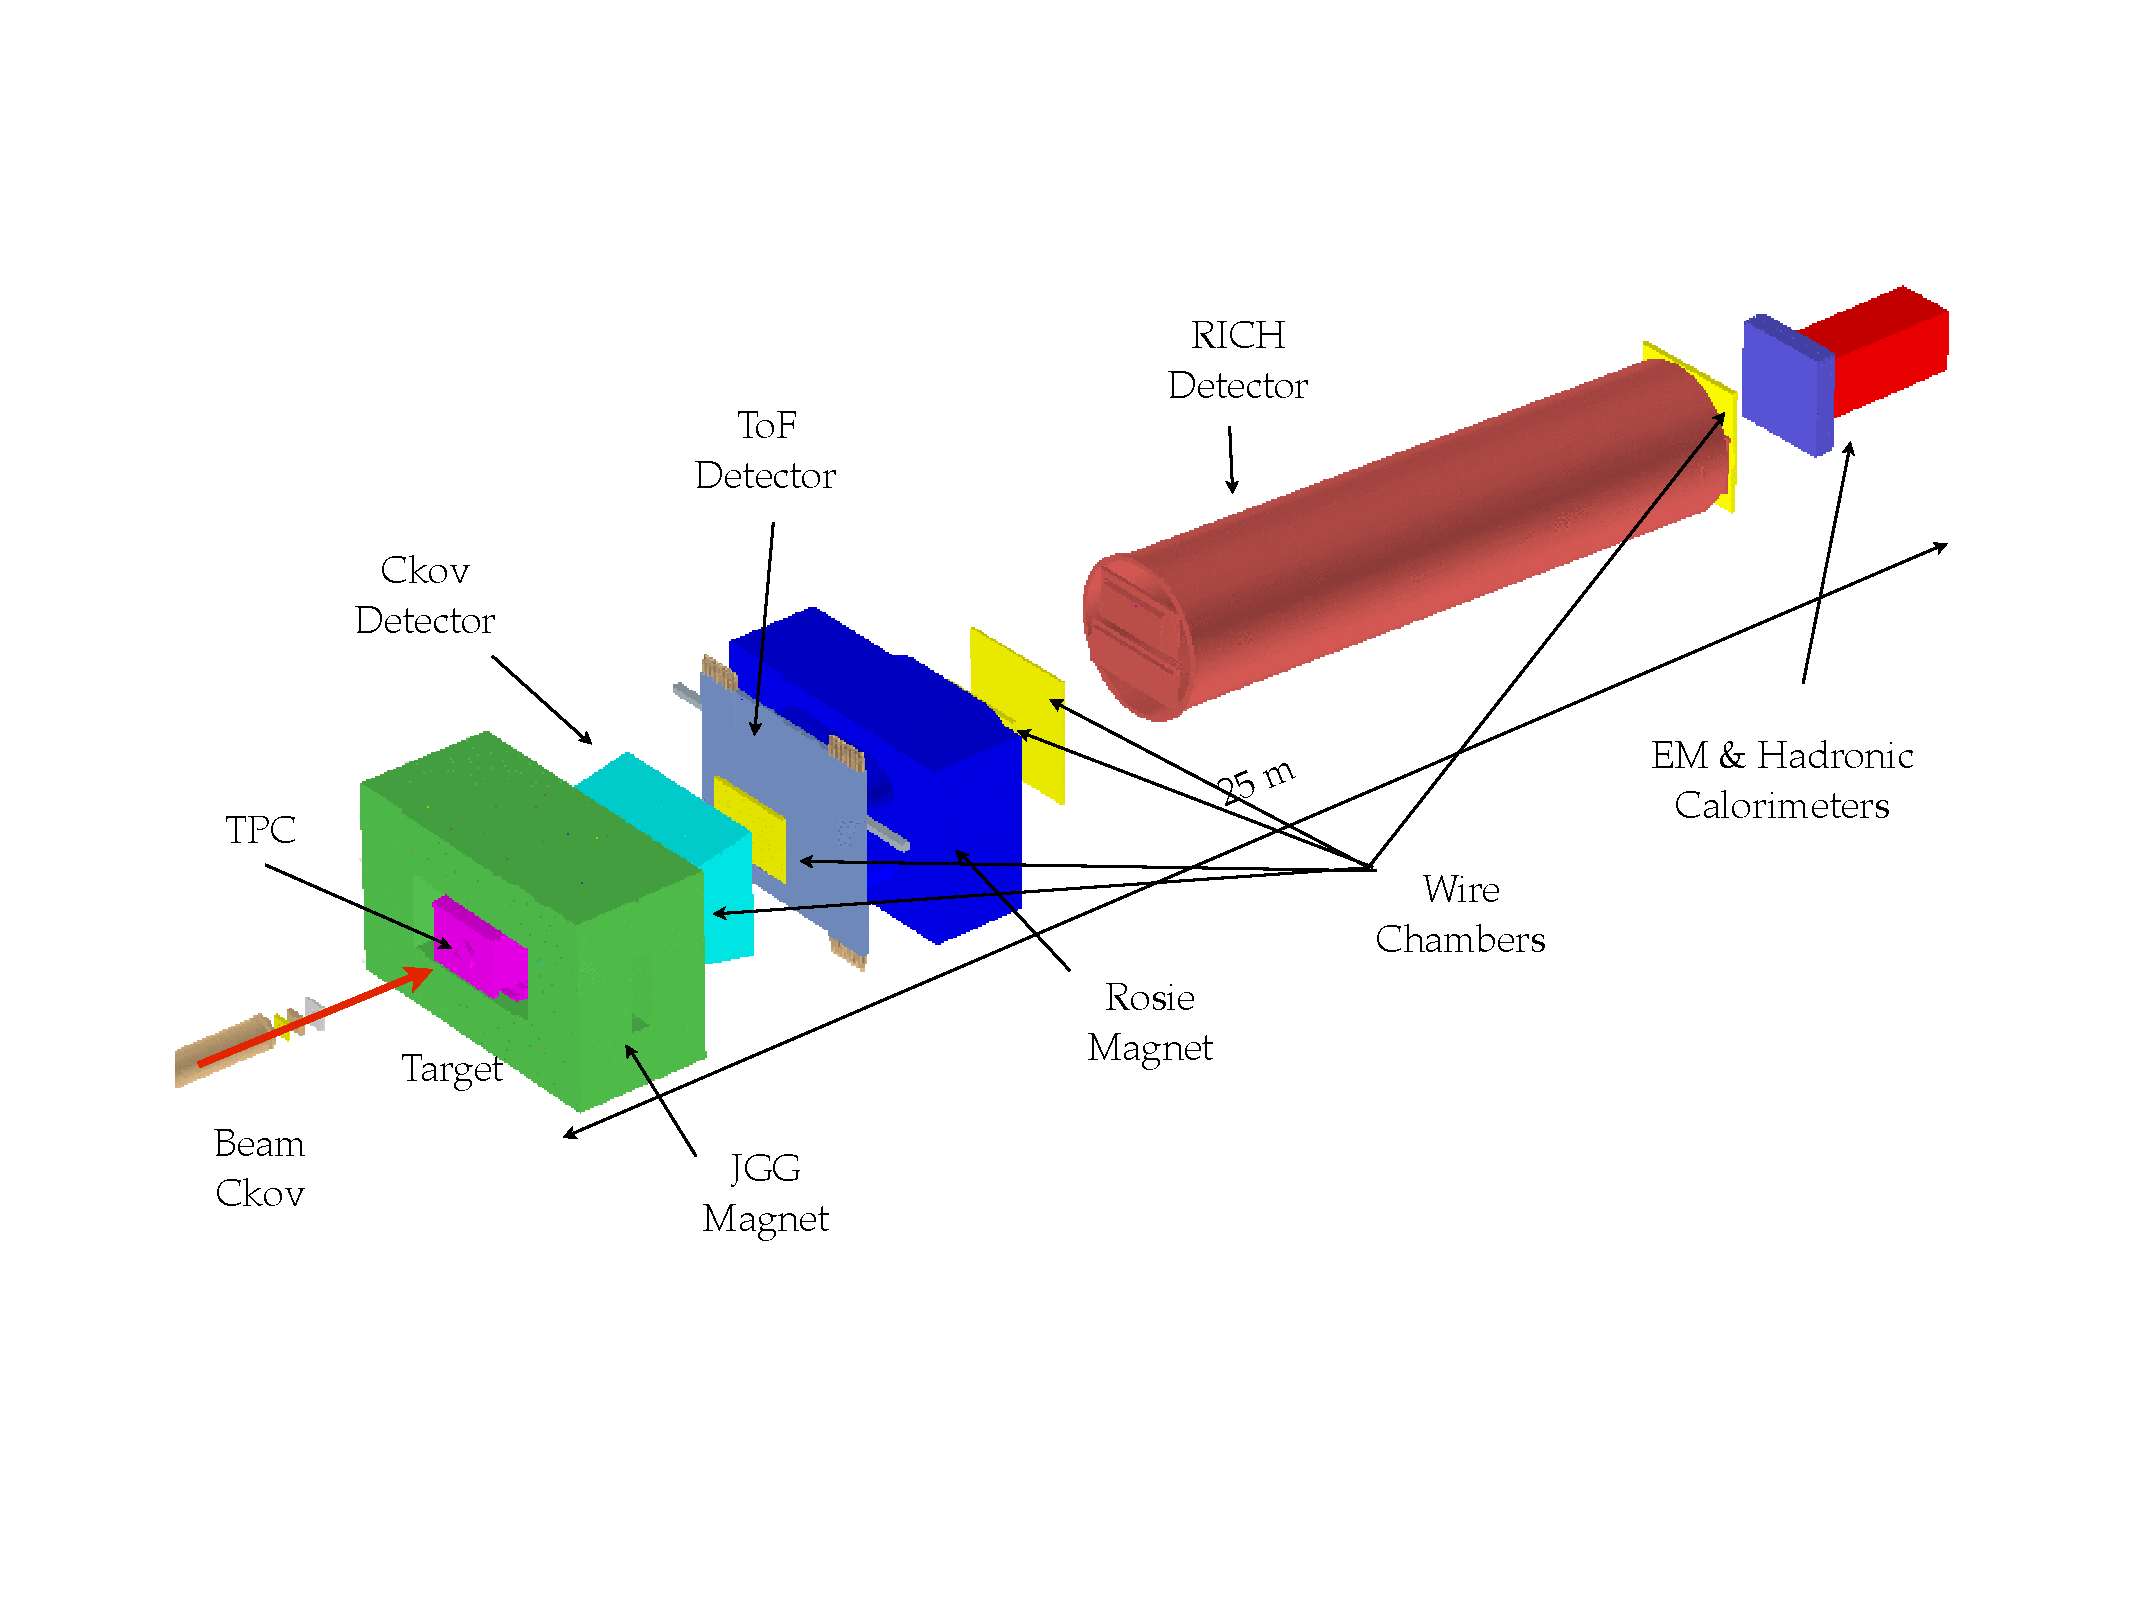
\includegraphics[width=0.45\textwidth]{MIPPSpectrometer}
   \caption{Schematic view of the MIPP spectrometer.}
   \label{fig:MIPPSpect}
\end{figure}

The MIPP Experiment used an open geometry 25 m long spectrometer, shown in Fig.~\ref{fig:MIPPSpect}, with two dipole magnets for momentum determination, a 1.5 m long time-projection chamber (TPC) located just downstream of the interaction region, and 3 multi-wire proportional drift chambers (MWPCs) and 2 proportional wire chambers (PWCs) located further downstream for particle tracking.  The TPC sits inside the most upstream dipole magnet, and targets are placed just upstream of the TPC.  Three wire chambers upstream of the target are used to track incident beam particles.  All tracking detectors have $\mathcal{O}$(mm) resolution in the transverse direction.  

MIPP was designed to provide particle identification (PID) with $2-3\sigma$ separation across the momentum range of a few hundred MeV to $\ge 80$ GeV using \dedx information from the TPC (0.2-1.2 GeV/c), a plastic scintillator-based time-of-flight (ToF) detector (0.5-2.5 GeV/c), a segmented gas Cherenkov detector (2-20 GeV/c) and a gas ring imaging Cherenkov (RICH) detector (4-80 GeV/c).  Electromagnetic and hadronic calorimeters are used to measure forward-going neutrons and photons\cite{ref:MIPPNeutron}.  The high multiplicities present in this data set complicate the use of the Cherenkov and ToF detectors, and this analysis focuses on data from the TPC and RICH detectors.  Data from the ToF detector are used to estimate backgrounds.

\section{Target and Incident Beam}
The NuMI target used in this measurement was a spare target that was eventually used by the NuMI complex after the MIPP data run.  The target consists of a $\sim 90$ cm long, 3 cm diameter aluminum tube encompassing 45(?) xx cm thick graphite slabs, adding up to two interaction lengths ($\lambda_L = 2$) of material.  The downstream end of the tube was inserted into the optics bay of the TPC, [x] cm away from the upstream end of the TPC active volume.  

The incident beam was 120 GeV/c protons, slow-extracted directly from the Main Injector (MI).  The MI beam was collimated such that the incident flux was reduced by 8 orders of magnitude, such that the rate of incident beam pileup in the target over the 16 $\mu s$ required to read out the TPC was reduced to a few percent.

\begin{figure}[t]
   \centering
   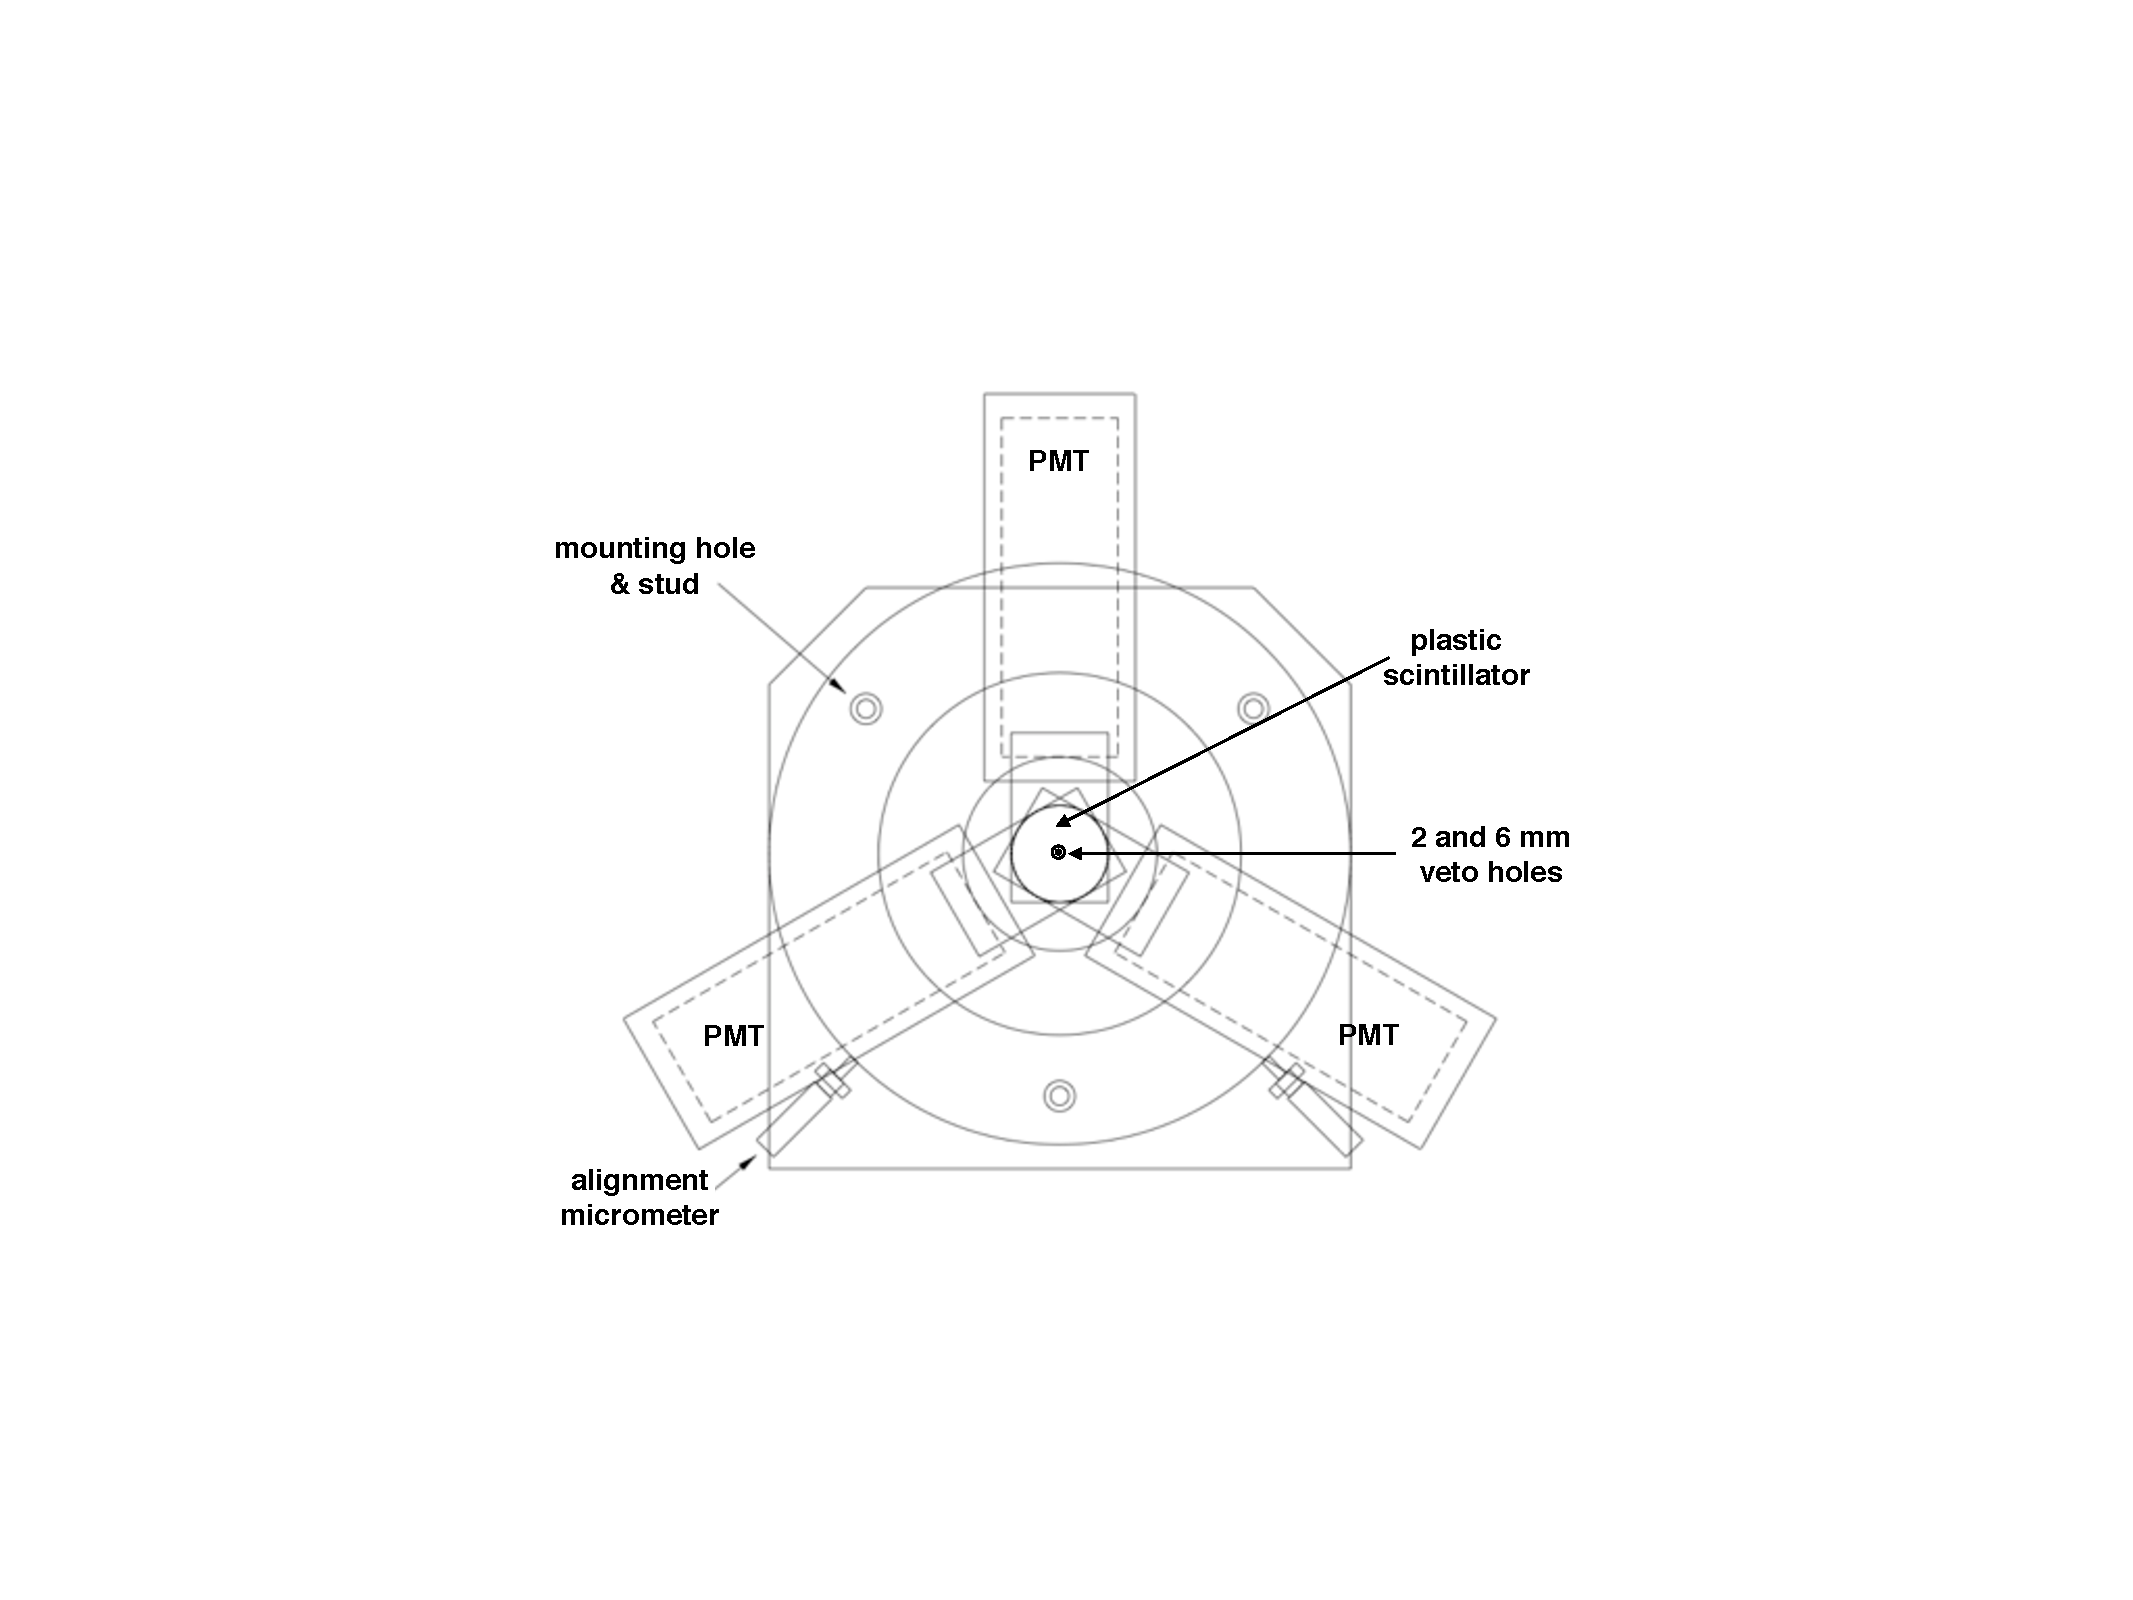
\includegraphics[width=0.45\textwidth]{NuMITrigger}
   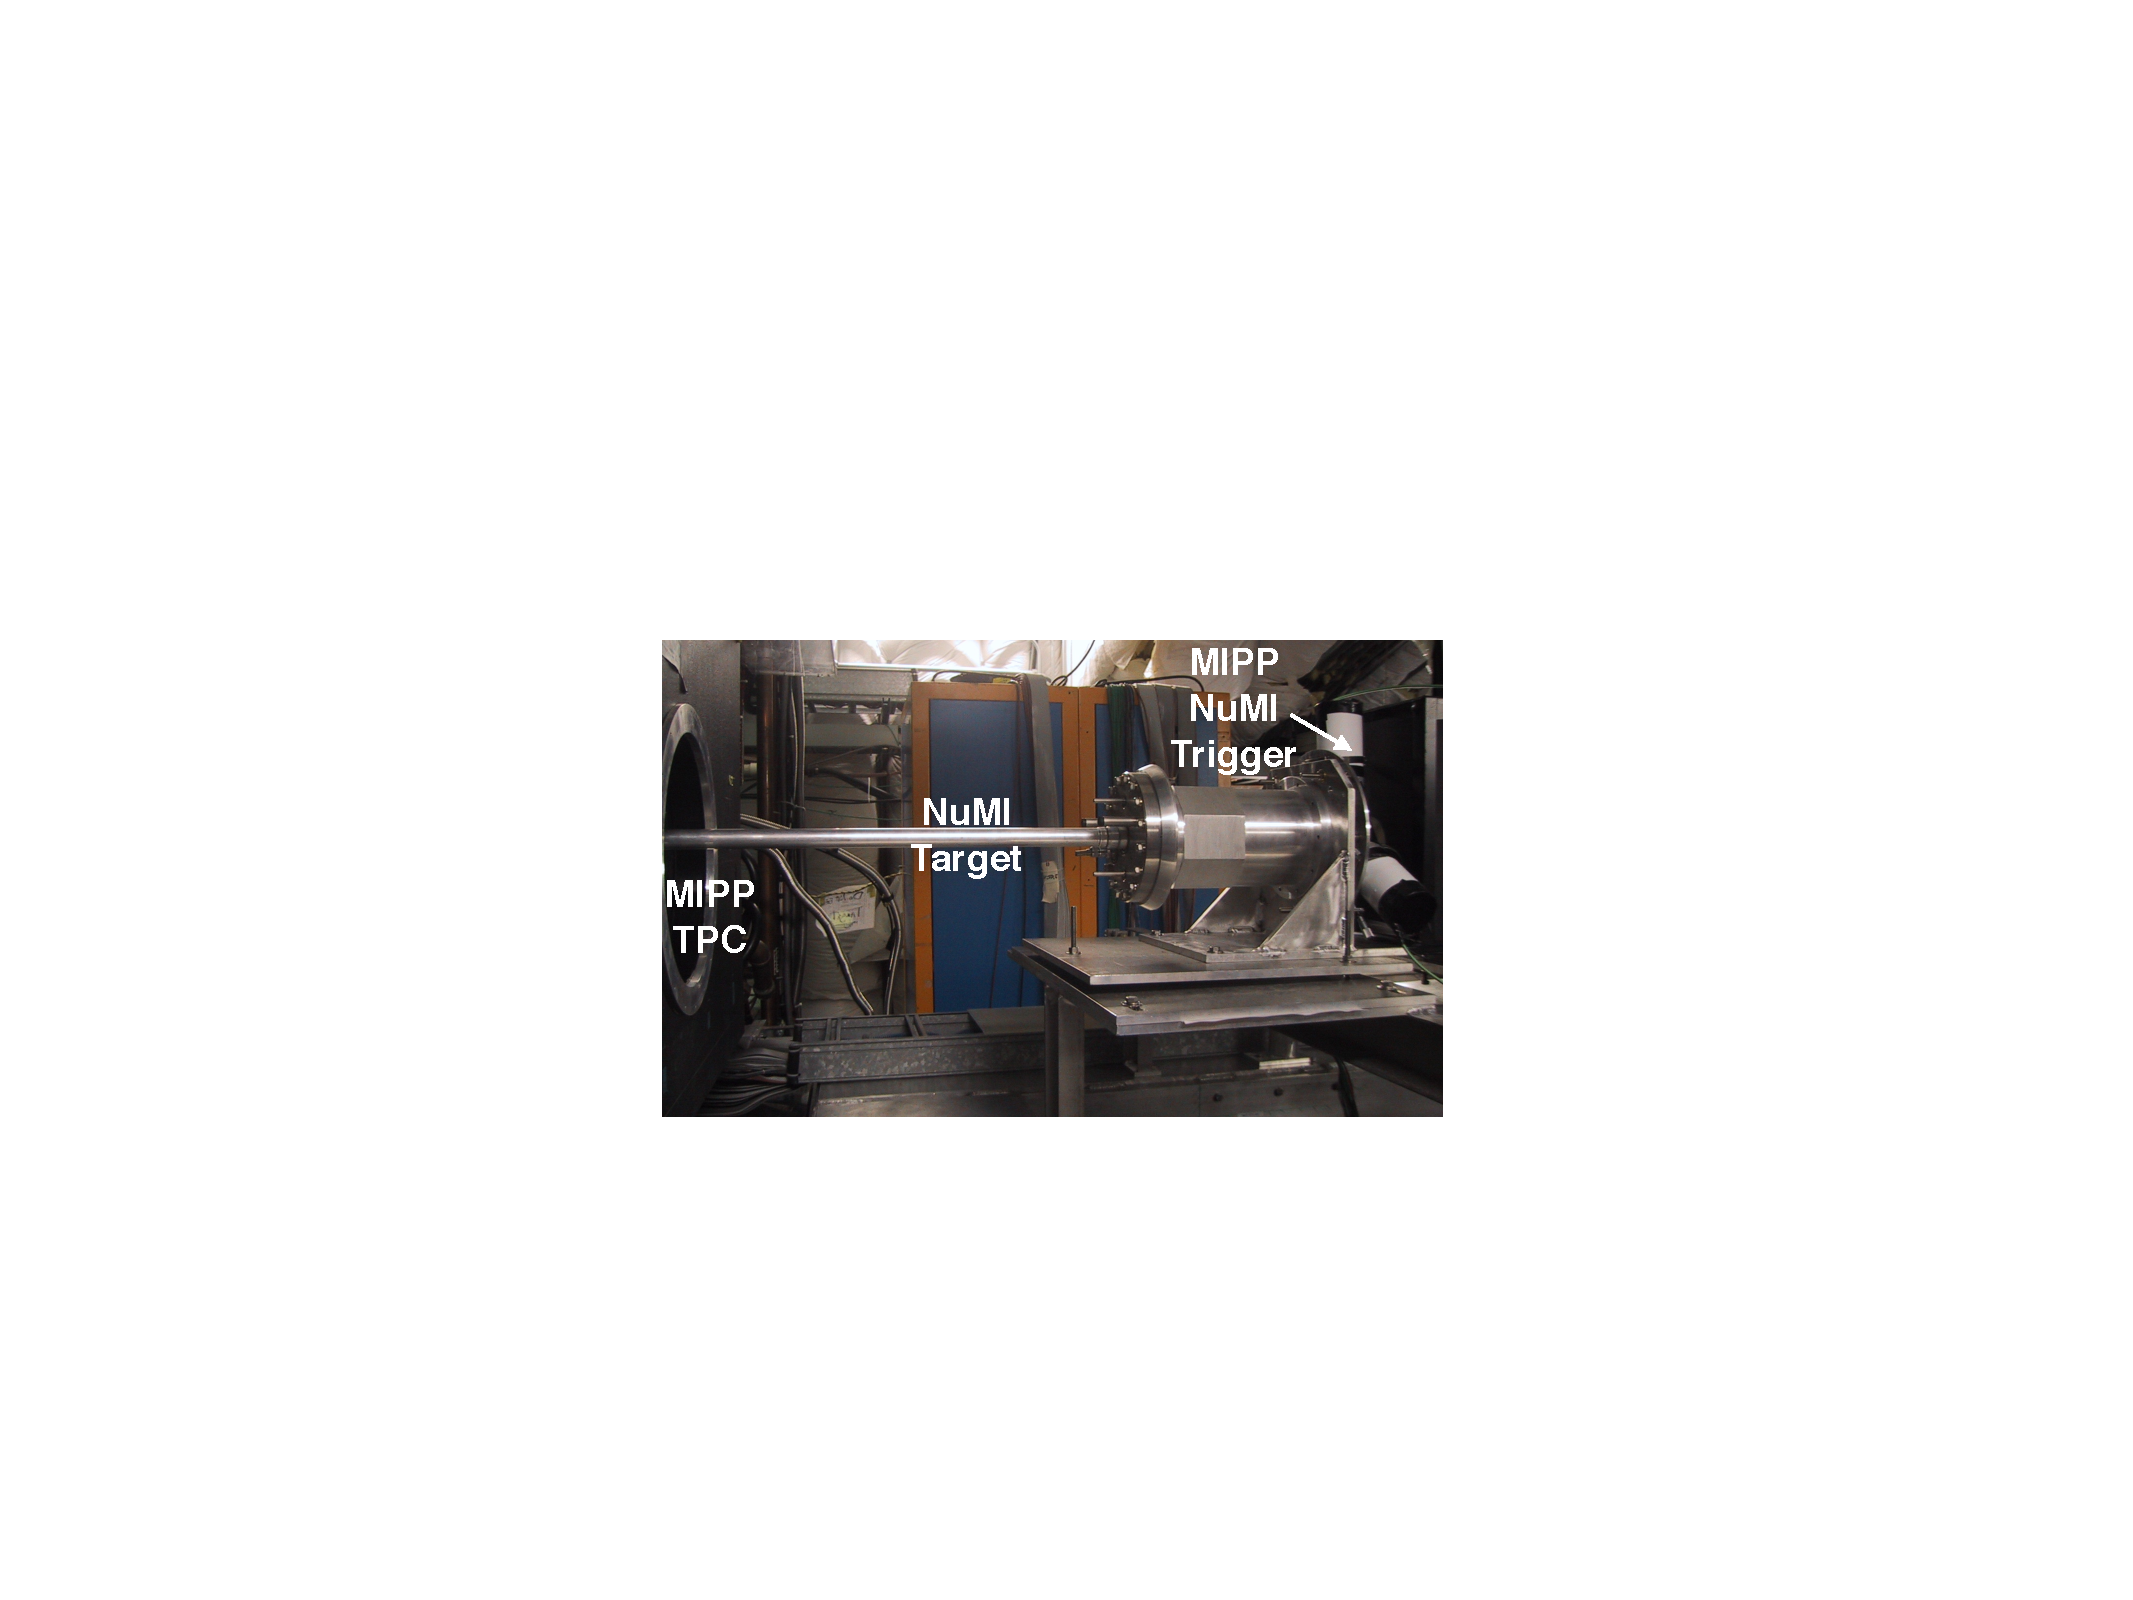
\includegraphics[width=0.45\textwidth]{NuMITargetInMIPP}
   \caption{Top: schematic of the MIPP NuMI trigger system.  Bottom: photo of the NuMI trigger mounted in the MIPP experiment, with the trigger system mounted on the upstream face of the target.}
   \label{fig:numitrigger}
\end{figure}

\begin{figure}[t]
   \centering
   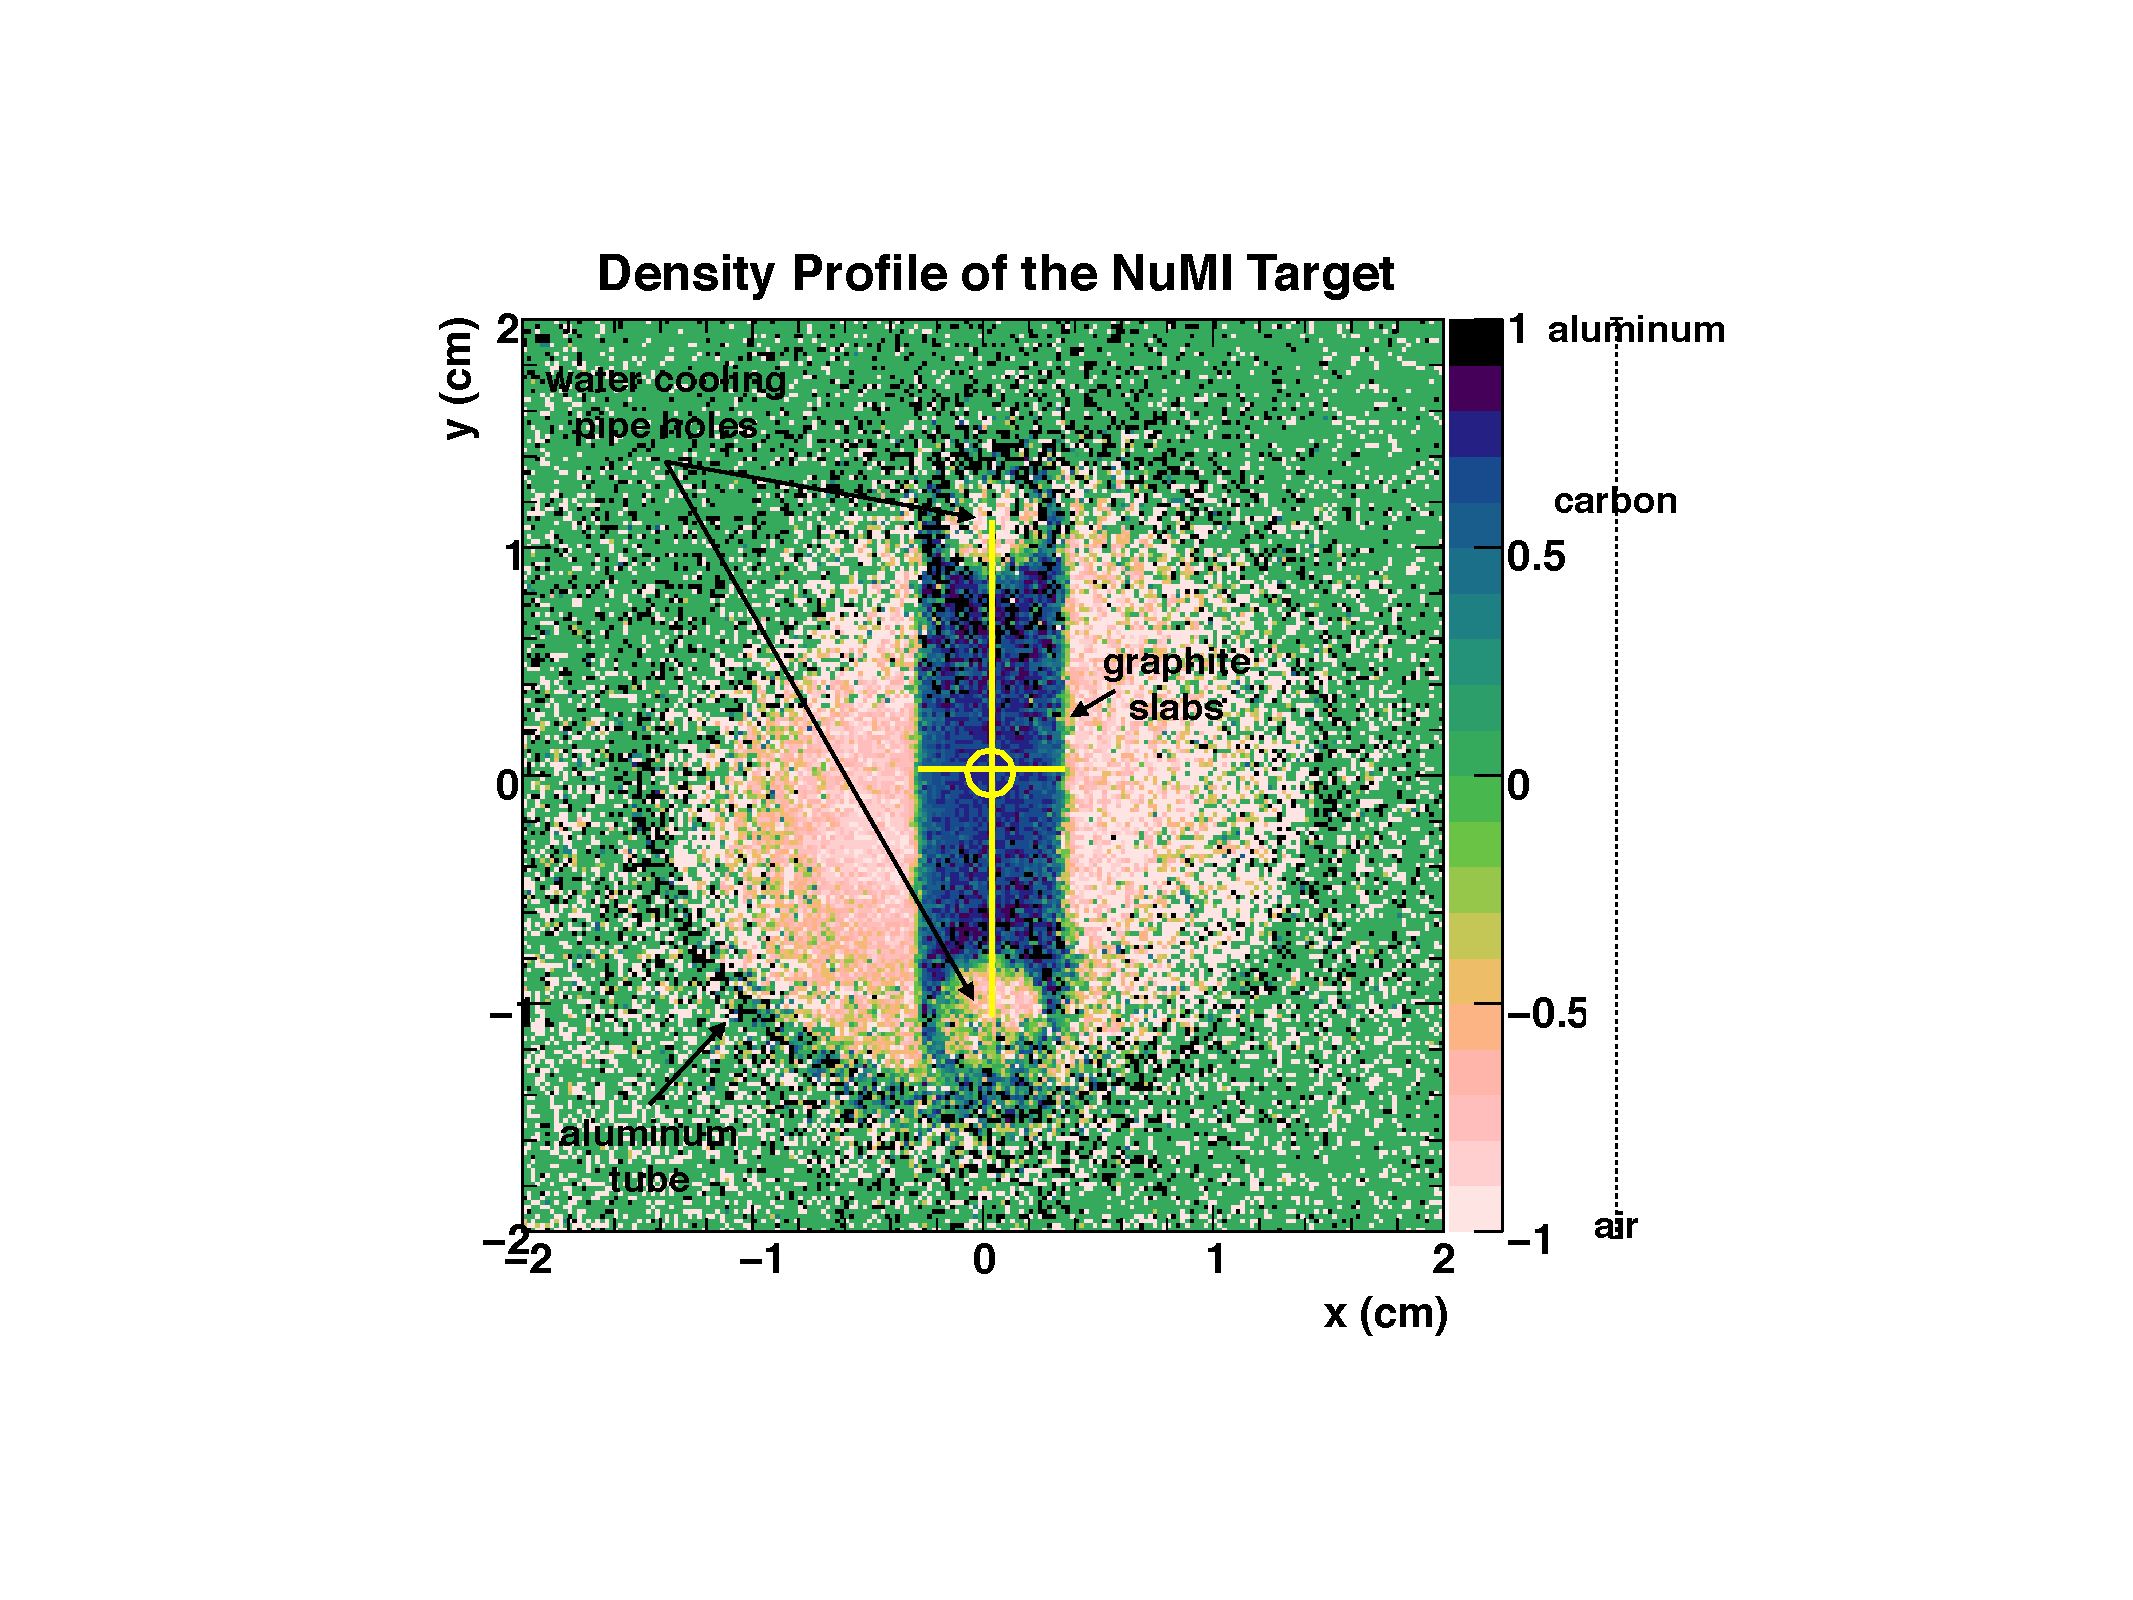
\includegraphics[width=0.45\textwidth]{trgt_profile2}
   \caption{Denisty profile of the NuMI target.  Cross-hairs represent the center
of the graphite slabs, and the circle represents the position of the 
2mm-trigger hole at the face of the target.}
   \label{fig:trgtprof}
\end{figure}

A trigger detector consisting of three thin ($\lambda_L < 0.5\%$) overlapping pieces of plastic scintillator was 
mounted on the upstream face of the NuMI target.  Light from each of the scintillator pieces was read out by a PMT.  
The middle and most downstream pieces of scintillator had holes 2 mm and 6 mm wide respectively drilled in the 
center.  A ``2-mm'' trigger was formed via a coincidence a signal from the upstream scintillator and the absence of signals 
from the middle and downstream scintillators.  A second ``6-mm'' trigger was defined by a signal from the upstream and 
middle scintillators and the absence of a signal from the downstream scintillator; this second trigger was prescaled
such that the full beam profile of protons on the NuMI target matched the profile in the NuMI beam.

A Fig.~\ref{fig:trgtprof} shows a density profile of the NuMI target.  
This radiograph is generated by looking at the normalized difference 
between the number of events where high and low multiplicities of secondary particles were produced.
Darker regions correspond to higher density materials; lighter region to less dense 
materials.  The graphite slabs located inside the NuMI target are clearly 
visible, with holes at the top and bottom where aluminum water cooling pipes 
run along the length of the target.  The outer aluminum tube containing the 
graphite and water cooling pipes is also visible.  The graphite slabs were 
actually found to be rotated $\sim 3^{\circ}$ about the z-axis; this rotation
has been removed in Fig.~\ref{fig:trgtprof}.  The data in the radiograph that define the edges of the 
NuMI target were taken opportunistically, while the MI beam was being aligned in the MIPP beamline.

The cross-hairs in Fig.~\ref{fig:trgtprof} represent the width and height
of the graphite slabs.  The positions of the cross-hairs were determined 
by fitting the edges of the $x$- or $y$-projection of the plot.  The measured
width of the graphite slabs is 6.36 mm; the technical specification of the NuMI
target claims the width of the slabs is 6.4 mm.  

Incident beam trajectories are reconstructed from hits in the three wire chambers upstream of the target.  The 
wire pitch of the beam chambers is 1 mm, and the wire chambers are separated by many meters, resulting in 0.2 mm track position reconstruction resolution at the upstream face of the target.  The circle near the center of 
Fig.~\ref{fig:trgtprof} represents the mean and width of the distribution of reconstructed beam positions on the 
face of the target for 2mm-triggered events.  The center of the circle is determined from Gaussian fits to 
peaks of the $x-$ and $y-$ beam position.  The beam center position is offset by 0.0452 mm
in the horizontal direction, and 0.174 mm in the vertical.  
%The beam position
%event cut requires the reconstructed beam position to be within 0.648 cm
%of the center of the graphite slabs (where the cross-hairs intersect).

\section{Simulation and Reconstruction}
\subsection{Simulation}
The MC generation of proton-NuMI target interactions in the MIPP experiment is a three-step process that uses 
the external packages, Fluka (v2005) for event 
generation (e.g., 120 GeV/c proton interactions on the NuMI target) and GEANT3 for particle trajectory tracking.  
The Fluka simulation generates primary, secondary, tertiary, etc. interactions of particles \emph{within} the target, 
and has a detailed geometric description of the NuMI target, the same geometry employed by the MINOS 
experiment.  Fluka tracks each particle produced in the target until it reaches the surface of the target, which is 
the outer edge of the Aluminum pipe encasing the graphite slabs of the target.  The next stage of the MC 
generation is GEANT3, which uses the output of the Fluka simulation as input, and tracks each particle taking 
into account multiple scattering, energy loss and decays through a detailed geometric description of the MIPP 
spectrometer.  GEANT ``hits'' are recorded in each detector volume until the particle either loses all energy or is 
well outside the volume of the MIPP spectrometer.  The last stage of the MC generation converts the GEANT hits 
to simulated digital signals, tuned to match data recorded in the experiment.

\subsection{Particle Trajectory Reconstruction}

\begin{figure}[t]
   \centering
   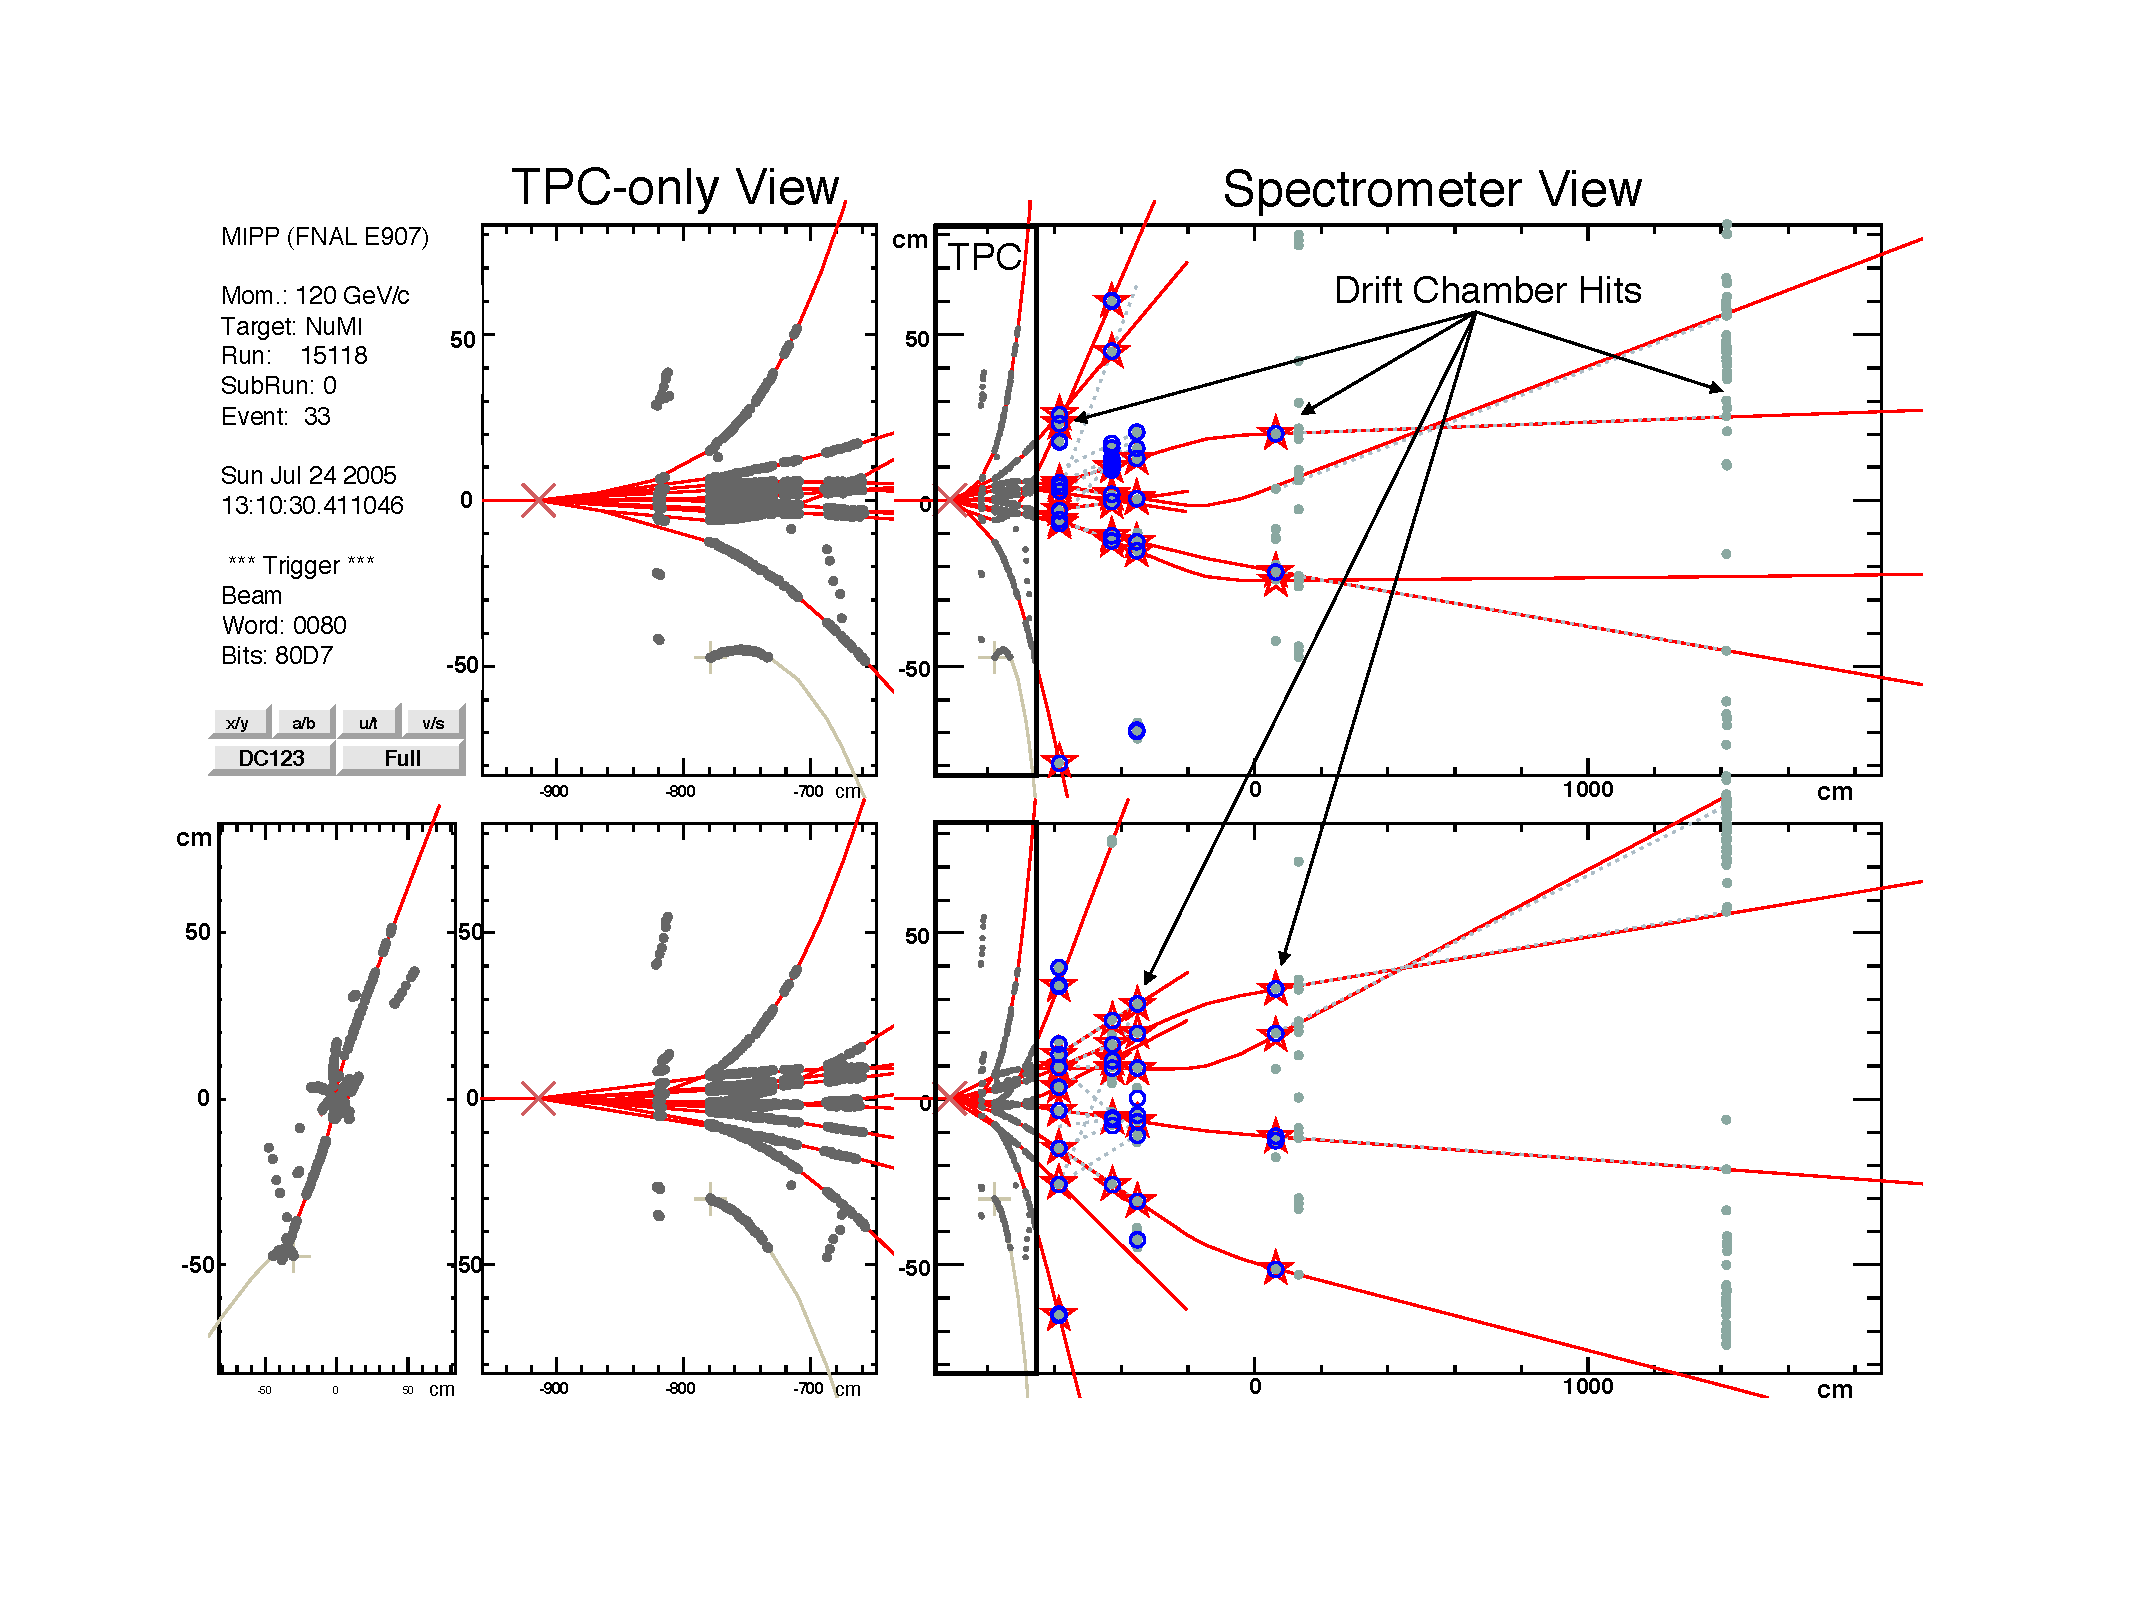
\includegraphics[width=0.45\textwidth]{NuMIEventDisplay}
   \caption{MIPP event display of real data showing the secondary particle reconstruction using recorded hits in the TPC and downstream drift and proportional wire chambers.}
   \label{fig:evd}
\end{figure}

The MIPP event reconstruction includes reconstruction of the trajectory of the primary beam particle using data 
from three wire chambers located upstream of the target, reconstruction of the secondary particles originating 
from the target, and matching the 
secondary particles to data recorded in specific channels in the ToF, Cherenkov, RICH and EMCal and HCal 
detectors.  The secondary particle trajectories are reconstructed by merging reconstructed track segments from 
hits in the TPC detector to track segments formed 
from hits in the downstream MWPCs and PWCs.  Fig.~\ref{fig:evd} shows an event display of NuMI target data recorded in the MIPP experiment; the gray points are the hits recorded in each detector and the red lines represent the reconstructed trajectories of the secondary particles emanating from the target.  The views in the top and bottom have been rotated to display the plane-view of hits in two orthogonal planes of the four downstream MWPCs.  The blue circles represent hits in each particular view, and the red stars represent hits in each view that have been associated with a reconstructed track.
%Vertices in this analysis, not shown in Fig.~\ref{fig:evd}, are constructed by first grouping tracks together that, given a large window, seem to be coming from a common 
%point, and computing a point that minimizes the distance of closest approach for all tracks.  Tracks are then either 
%rejected or added in an iterative process that decreases the window size for 
%associated tracks until a minimum window size is reached.  
In the analysis of the NuMI target data, Monte Carlo simulation studies indicate that the momentum resolution is $3-5\%$, and the transverse momentum resolution is $<20$ MeV/c for all momenta. 

\subsection{Particle Identification}

\begin{figure}[thp]
   \centering
   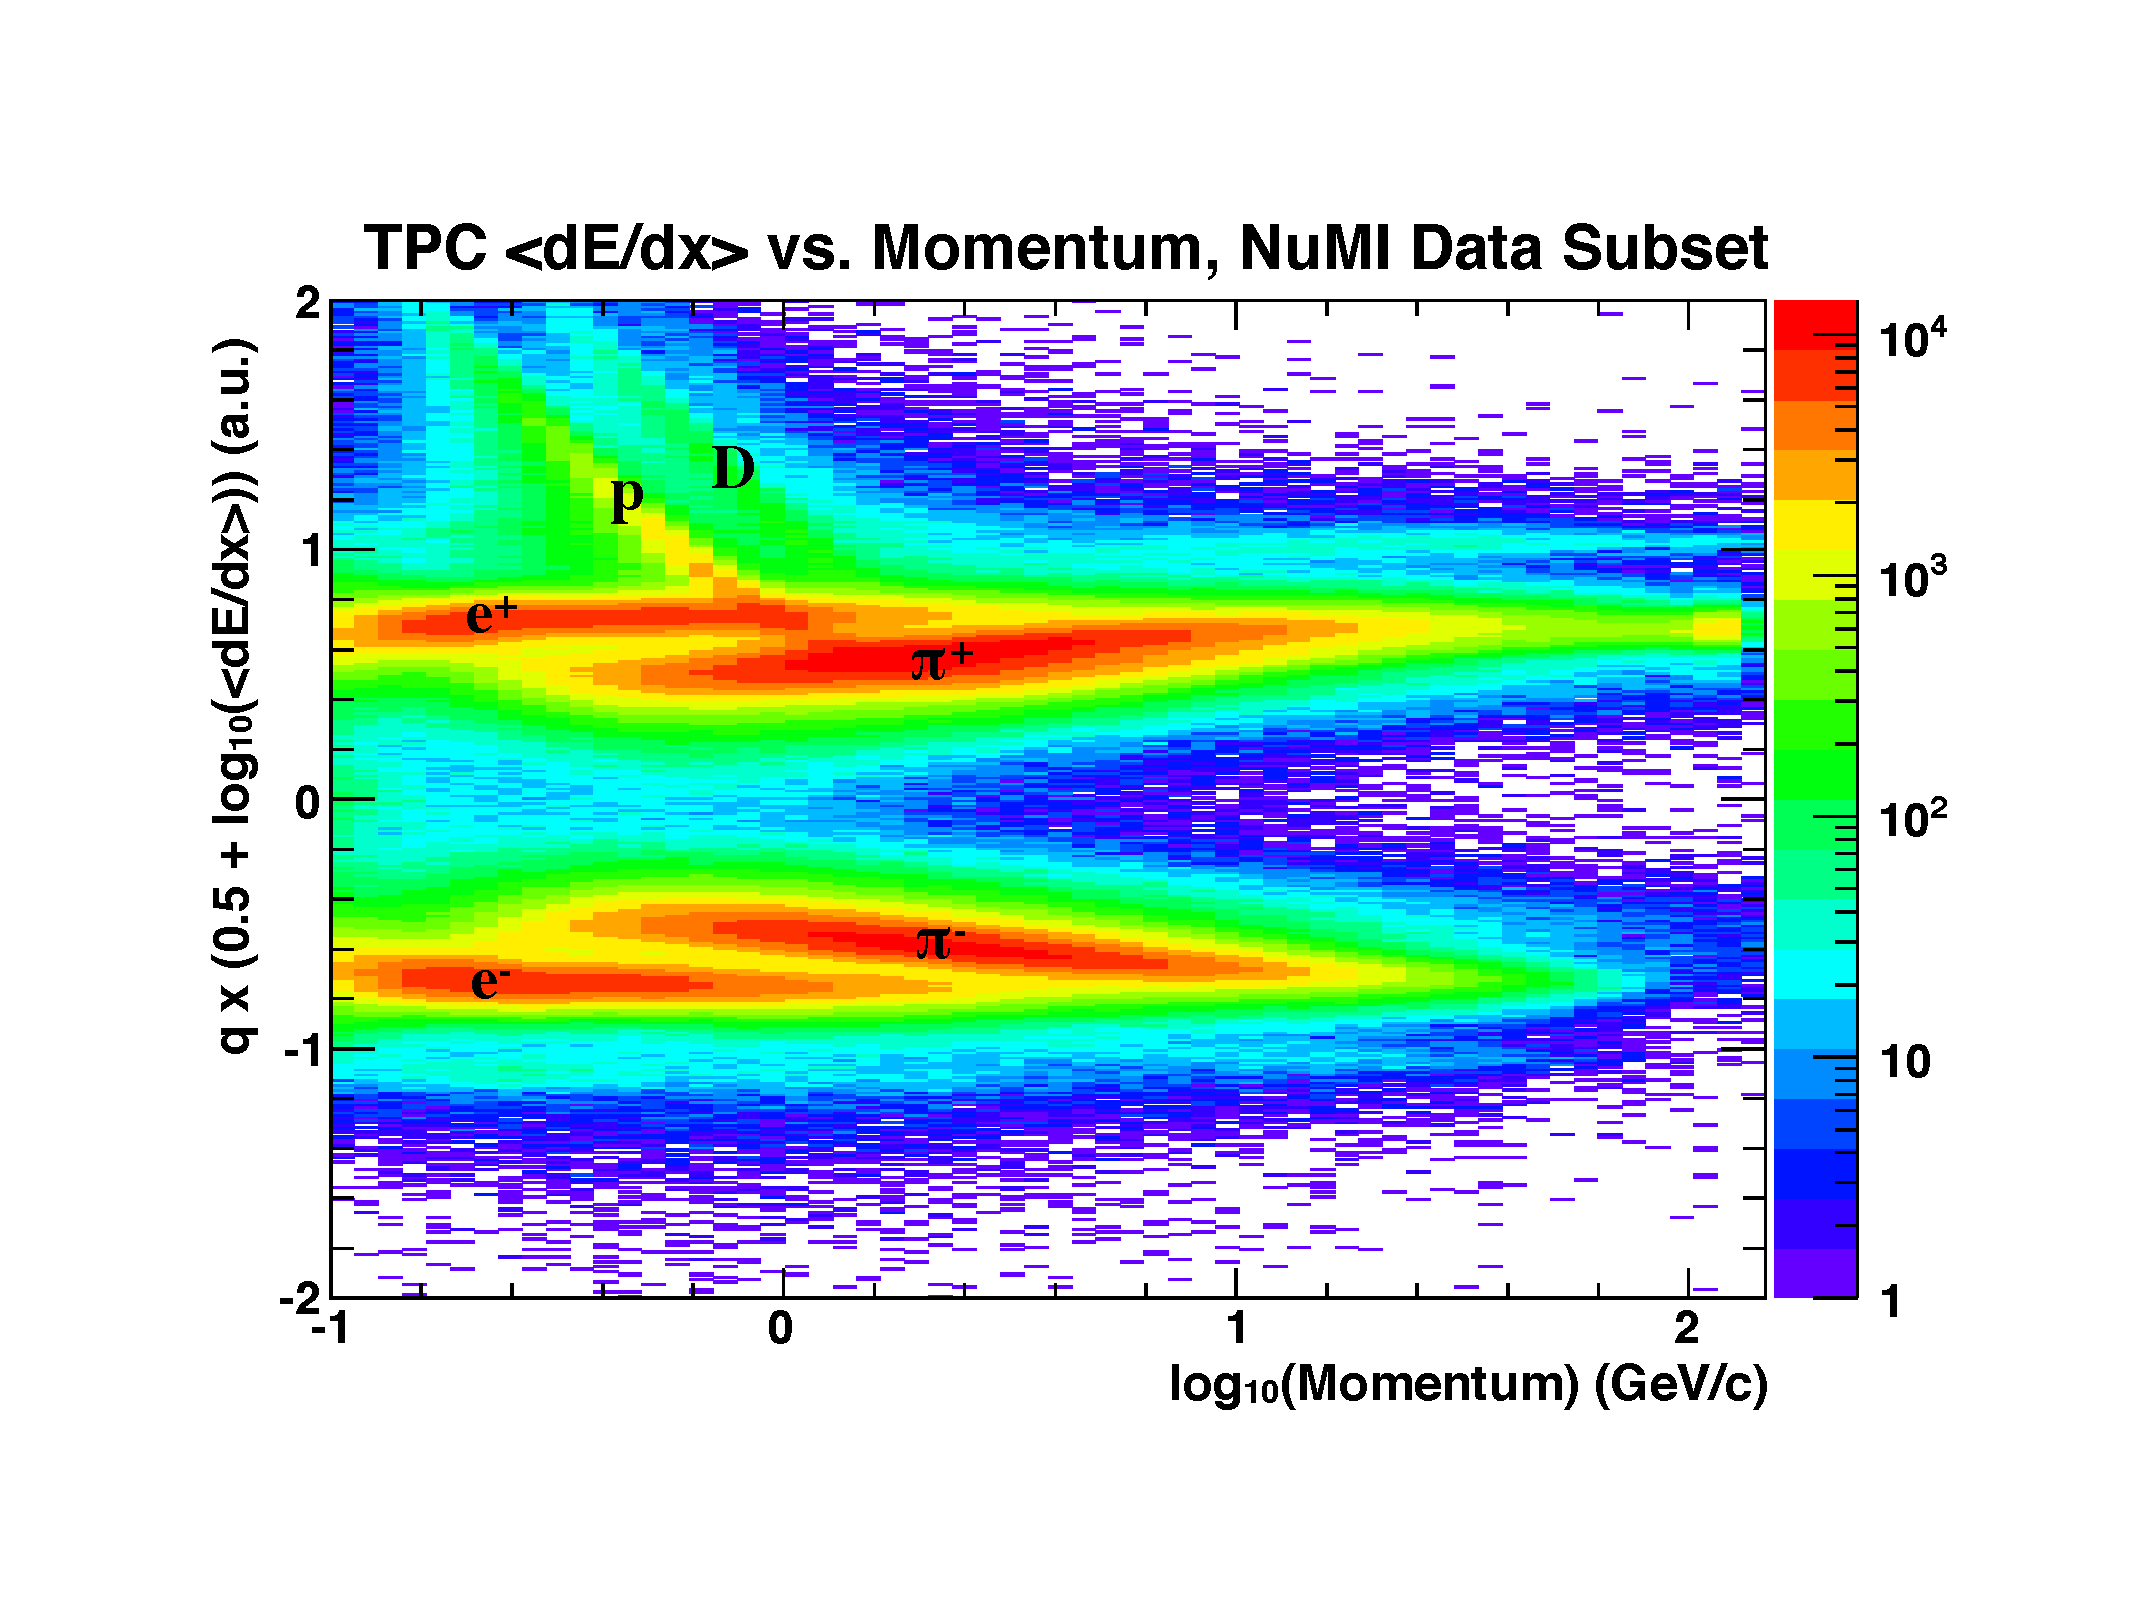
\includegraphics[width=0.45\textwidth]{NuMITPCdEdx}
   \caption{Distribution of measured charge $\times$ \dedx as a function of $\log_{10}(p)$.  Colors represent the density of particles at the reconstructed momentum and \dedx, and bands for different particle types are clearly visible.}
   \label{fig:dedxVsMom}
\end{figure}

The \dedx is determined for every reconstructed track from TPC hits based on the charge recorded on 8 mm $\times$ 12 mm charge-sensitive pads in the readout-plane of the TPC.  Time-dependent corrections, relevant on the order of hours to days, are applied to the data to account for changes in water-vapor and oxygen contamination in the TPC gas.  The TPC data are normalized such that \dedx = 10 for pions between 500-550 MeV/c.  Tracks in this analysis had 20-90 associated TPC hits providing clean separation of $\pi$ and $p$ between 0.2 and 1.2 GeV/c.  

Reconstructed tracks are matched to hits recorded in the ToF.  Temperature-dependent and cross-talk corrections are applied to the ToF data, and improve the timing resolution of the detector from 1.2 ns to $<400$ ps.  As a result, the ToF data provide $\pi-p$ separation up to about 2 GeV/c.  However, due to the high multiplicities of secondaries in the NuMI data set, many particle trajectories pass through the same ToF channels and it is impossible to disentangle the particles in the ToF data.  Therefore only a subset of ToF data are usable.  

%The Cherenkov detector is made of 96 mirrors which reflect the light produced inside the gas volume onto PMTs.  Data-driven calibrations indicated that $<10$ photo-electrons were typically measured for a $\beta=1$ particle.  Furthermore, this detector also suffers from the same high multiplicity problem as the ToF; approximately 50\% of all particles passing through the detector coming off the NuMI target share light with another particle.  In this analysis, data from the Cherenkov detector are not used.

Particles in the RICH detector produce light cones which are reflected to form a ring of light on an array of $\sim2300$ 1/2" PMTs.  The high segmentation of the RICH detector allows for multiple rings to be clearly distinguished and matched to reconstructed tracks, therefore the high multiplicities of secondaries is not an issue for this detector.  The RICH detector allows for clean pion identification beginning above 4 GeV/c, and clean kaon identification above 20 GeV/c.

\begin{figure}[thp]
   \centering
   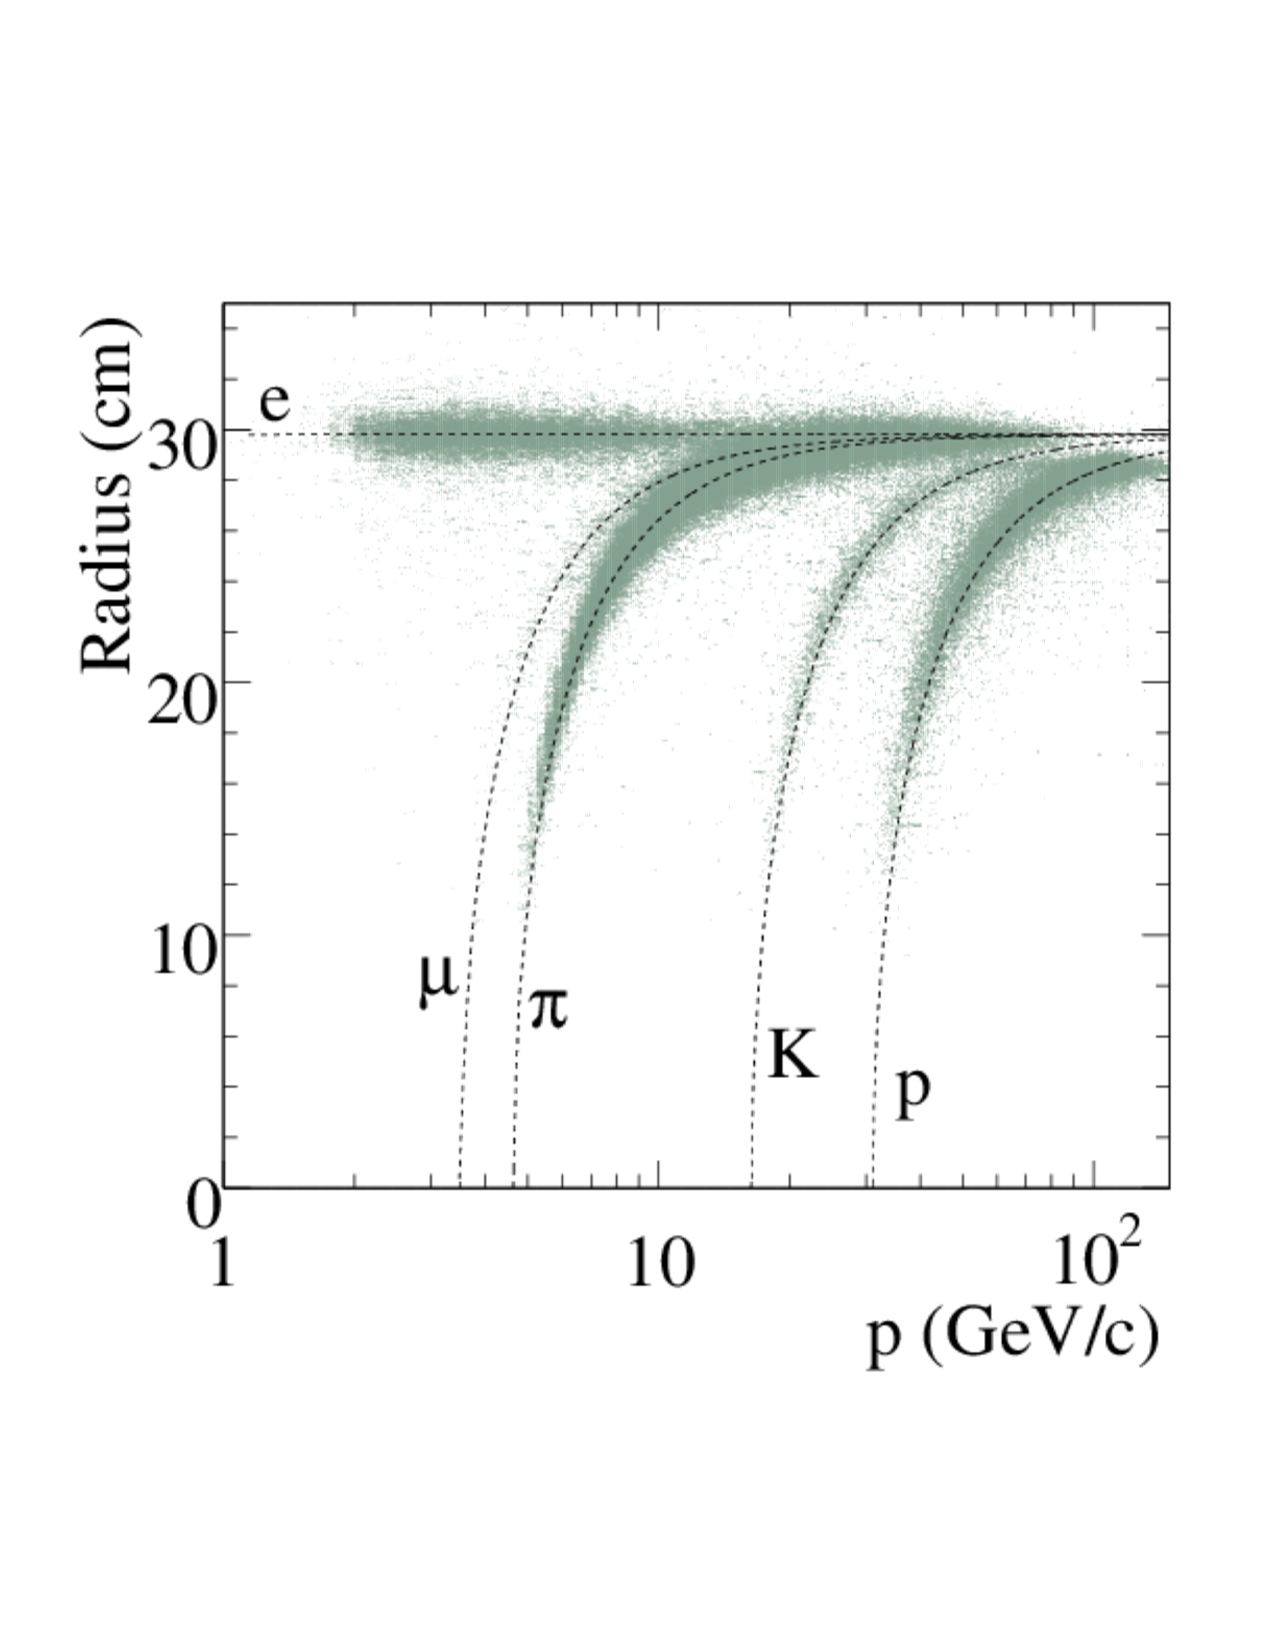
\includegraphics[width=0.45\textwidth]{RICHNuMIPosTrack2}
   \caption{Reconstructed RICH ring radius as a function of track momentum for positively charged tracks in the NuMI target data set.  Gray points are measurements for individual tracks, and the predicted bands for the different particle types are superimposed as dashed lines.}
   \label{fig:richRingVsMom}
\end{figure}


\section{Analysis}

This analysis is a measurement of the pion yield off the NuMI target, $N_\pi$\pzpt.  Yields will be extracted from TPC \dedx and RICH $m^2$ distributions.  Corrections will be applied to each measurement to account for spectrometer geometric acceptance, track reconstruction efficiency, PID detector geometric acceptance and PID detector efficiency:

\begin{equation}
N_\pi(p_z,p_T) = \frac{N_\pi^\mathrm{meas}}{\epsilon^\mathrm{spect}_\mathrm{accept} \times \epsilon^\mathrm{reco}_\mathrm{eff} \times \epsilon^\mathrm{PID}_\mathrm{accept} \times \epsilon^\mathrm{PID}_\mathrm{eff}}
\end{equation}

In general, unless otherwise noted, the measurement and calculations of corrections to be applied to the data are done for positive and negative particles separately.

\subsection{Momentum Calibration}
A small, $< 1\%$ correction, based on a comparison between reconstructed and true momenta of MC tracks, is applied to 
the reconstructed momenta of tracks through the MIPP spectrometer to account for energy loss and scattering, as well as biases introduced by the reconstruction algorithm.  The overall momentum scale is calibrated using reconstructed primary beam protons that pass through the target in data, and reconstructed K$^0$ mass from oppositely charged pairs of tracks produced off the target in data.  The primary beam was found to agree with the expected 119.6 GeV/c from the Main Injector.  The peak of the distribution of reconstructed K$^0_\mathrm{s}$ invariant masses from pairs of oppositely charge tracks was found be 0.85\% lower than the PDG value.  The momenta of tracks that contribute to the K$^0$ mass peak is peaked around 1 GeV/c.  A linear interpolation between these two measurements, one at 1 GeV/c (0.85\% offset) and the other at 120 GeV/c (0\% offset) is used to correct for absolute momentum.

%\subsection{PID Detector Calibration}
\subsection{Event Selection}
Event selection in this analysis is designed to reject events with multiple incident beam particles (protons)  while requiring that the beam is centered on the NuMI target.  We require exactly one reconstructed incident beam track from data recorded in the upstream beam wire chambers, a reconstructed beam track time that falls within the expected 13.4 ns-wide window from the accelerator RF bucket, %limited ``out-of-time'' activity in the TPC, 
and a reconstructed beam track position that falls within 0.648 cm of the center of the upstream face of the target.   
Because the readout of the TPC data lasts 16 $\mu s$, particles traversing the center of the TPC many $\mu s$ before [after] the event trigger will have a shorter [longer] recorded time and therefore appear to be well below [above] the center of the TPC.  Events with an excess of TPC tracks appearing at the top or bottom of the TPC were rejected, and MC studies indicate the rejection of these events have a negligible bias ($< 0.03\%$ MC events are rejected, whereas 5.7\% data events are rejected).

\subsection{Binning}
The yields of secondary pions produced in the target are measured in bins of $p_\mathrm{z}$ and $p_\mathrm{T}$ chosen to keep the statistical uncertainty in each bin to less than $5\%$ while not exceeding the momentum resolution of the spectrometer in each bin.  So far no physics motivation has been identified to use finer binning at lower momentum.  A total of 76 bins are defined in this analysis, however due to limited statistics in some bins, pion yields are reported for 60 bins covering 300 MeV/c - 80 GeV/c and 4 bins from 0 to 2 GeV/c in $p_\mathrm{T}$ .

\subsection{Efficiency and Acceptance Corrections}
Geometric acceptance and track reconstruction efficiency corrections are determined using MC simulations which have detailed descriptions of the target and spectrometer and detector geometries.  The combined geometric acceptance of the spectrometer and the track reconstruction efficiency are shown in Fig.~\ref{Fig:RecoEff} as a function of \pzpt.  Fig.~\ref{Fig:PIDAccept} shows the geometric acceptance of the PID detectors.  The color of the boxes indicates the scale on the z-axis of the plots, where 100\% efficiency or acceptance is red and violet represents 0.  Both plots show results for negative particles; positively charged particles have very similar efficiencies and acceptances.  All reconstructed tracks have a measurement of \dedx, therefore at low momentum where the \dedx is used for PID, and the acceptance is 100\%.  On the other hand, measurements in the RICH detector require particles to traverse the length of the detector, and so not all particles satisfy this condition.  This is particularly true for lower momentum particles and is the reason for the low acceptance in the RICH PID detector at low momenta.  The white bins in Fig.~\ref{Fig:PIDAccept} indicate those bins for which we do not have a means to identify pions.

\begin{figure}[t]
  \centering
  \subfigure[Combined geometric acceptance and track reconstruction efficiency.  ]{\label{Fig:RecoEff} 
  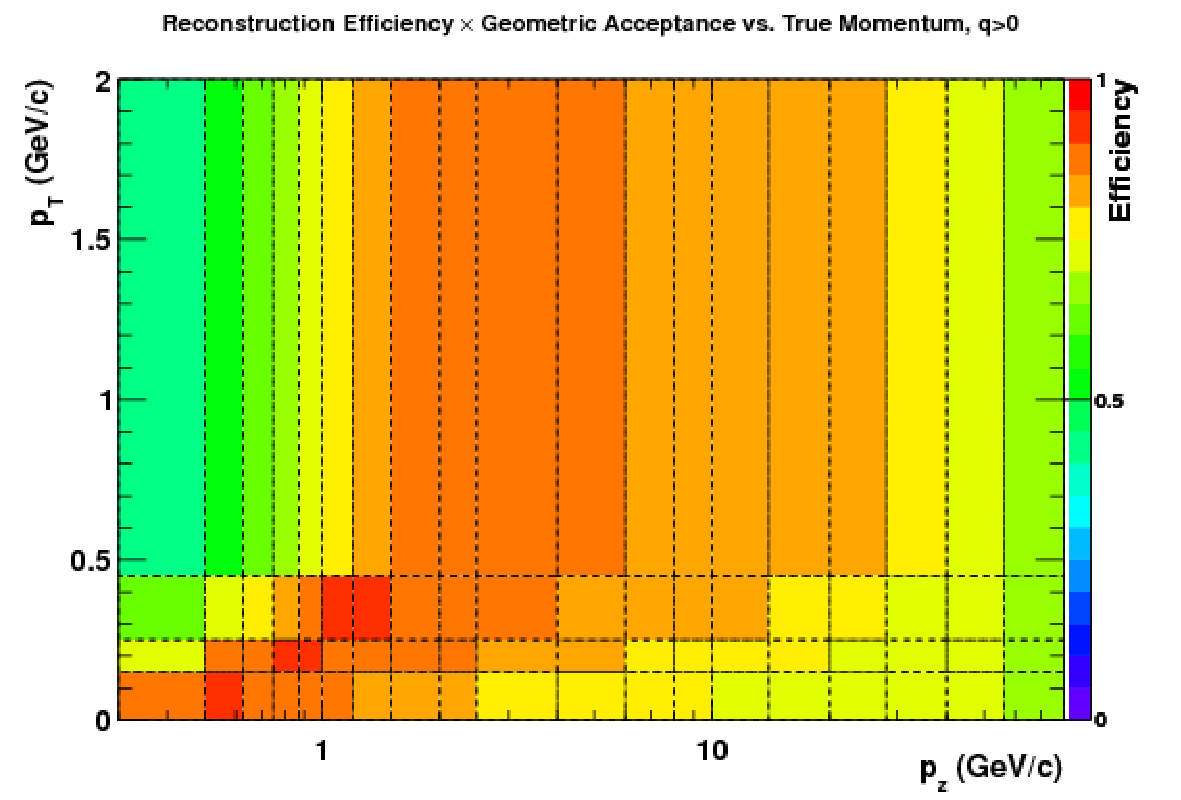
\includegraphics[width=0.47\textwidth]{RecoEff.pdf}}
  \subfigure[Acceptance corrections for the TPC and RICH particle identification detectors.]{\label{Fig:PIDAccept}
  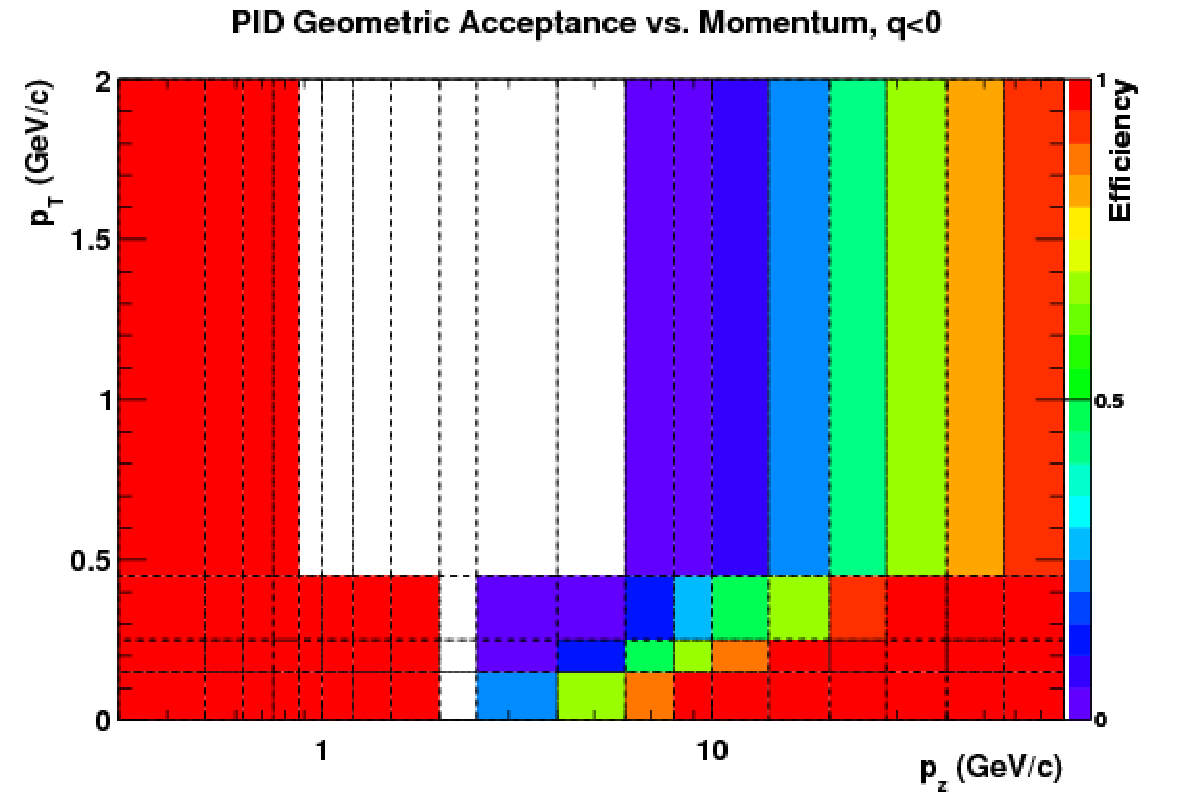
\includegraphics[width=0.47\textwidth]{PIDAccept.pdf}}%
  \caption{Acceptances and reconstruction efficiencies as a function of \pzpt as determined from MC simulation.  The numbers in the boxes refer to a bin number, the colors represent the efficiency (red=100\%, green=50\%).}
  \label{Fig:AcceptPlots}
\end{figure}

\subsection{PID Detector Measurements}

\subsubsection{TPC Measurements}
Every reconstructed track has a corresponding measurement of \dedx.  In any given slice of total momentum, the 
distribution of log(\dedx) for any particle type is nearly Gaussian.  The log(\dedx) distributions in narrow bins of \pzpt are 
very nearly Gaussian.  We therefore fit the $q \times$ log(\dedx) distributions to a sum of six Gaussians, 2 peaks 
each for $e, \pi$ and $p$.  The distribution is centered about zero by construction, so the 
means of the positive and negative of each particle simply has a sign flip.  Furthermore, the width of the positives 
and negatives of each particle type is assumed to be identical.  Therefore the fit function to these distributions 
has 12 free parameters, 3 means, 3 widths, and 6 amplitudes, rewritten as ratios with respect to the amplitude of the pion peak:
\begin{eqnarray}
N(x) &  =  & A_{\pi^+}\left[f^{+}_{e\pi}G_e(x) + G_\pi(x) + f^+_{p\pi}G_p(x)\right]  + \nonumber \\
& & A_{\pi^-}\left[f^{-}_{e\pi}G_e(x) + G_\pi(x) + f^-_{p\pi}G_p(x)\right]  
\end{eqnarray}
where 
\begin{equation}
G_i = \exp\left(\frac{(x-x_i)^2}{2\sigma_i^2}\right)
\end{equation}
is the Gaussian function for each particle type.  $x$ is the measured value of $\log_{10}$\dedx, $x_i$ is the 
mean, $\sigma_i$ is the width, $A_{\pi^\pm}$ is the fit amplitude of the pion peak, and $f_{e\pi}$ ($f_{p\pi}$) is the 
ratio of the electron (proton) peak to the pion peak.

One feature of the \dedx distributions is that at higher momenta (e.g., above $\sim 1.2$ GeV/c), large fractions if not all of the proton peak falls under the pion peak and the fit to 6 peaks either fails (the fitted proton peak becomes unphysically large or small).  However, in this range, the protons are clearly distinguished from pions and electrons in the ToF.  Fig.~\ref{fig:ToFvsTPC} shows the reconstructed $m_\mathrm{ToF}^2$ of tracks with isolated hits in the ToF vs. the \dedx of these tracks.  The protons are very clearly visible in the ToF (e.g., $0.5 < m_\mathrm{ToF}^2 < 1.2$ GeV${^2}$/c$^{4}$), whereas these protons fall under the pion and electron \dedx peaks on the x-axis.  The relative amount of protons is determined from these data by assuming all particles with 
$m_\mathrm{ToF}^2$ between 0.5 and 1.2 GeV${^2}$/c$^{4}$) is a proton, and fitting the \dedx distributions for tracks with ToF $m_\mathrm{ToF}^2$ below 0.5, and is used as a constraint to fits of the TPC \dedx distribution for tracks that do not have isolated hits in the ToF for bins with momentum greater than 0.88 GeV/c.

\begin{figure}[!ht] %  figure placement: here, top, bottom, or page
   \centering
   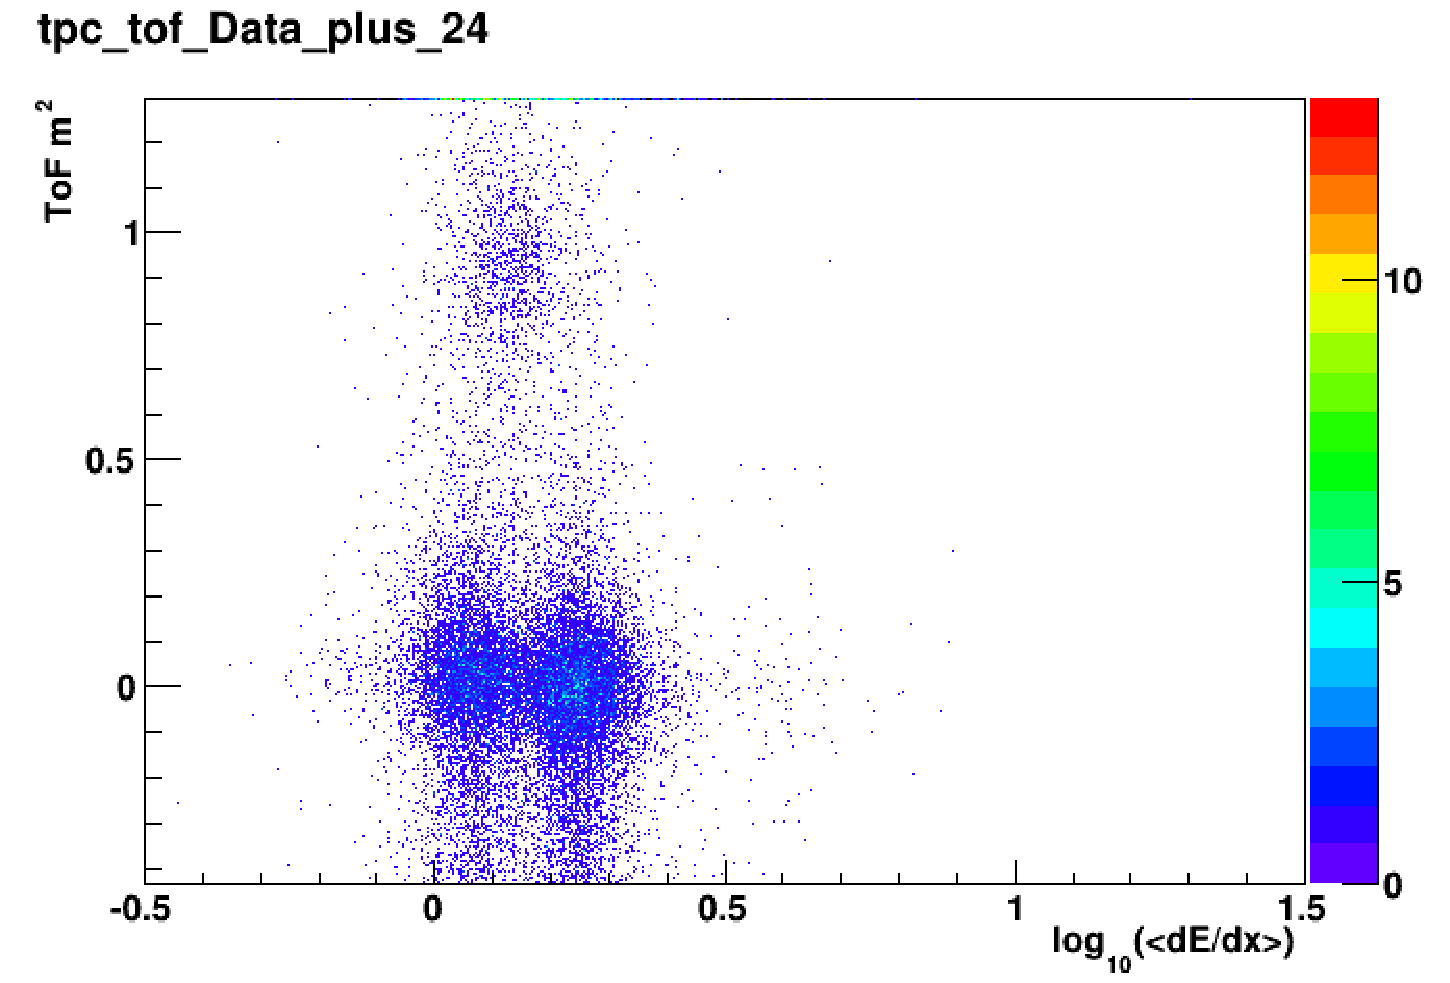
\includegraphics[width=0.45\textwidth]{tpc_tof_Data_plus_24_zoom} 
   \caption{ToF $m^2$ vs.~TPC \dedx for $1.2 \le p_z < 1.5, 0.0 \le p_T < 0.15$ GeV/c for tracks with isolated hits in the ToF.  Note that the protons are clearly distinguished from visible in the ToF, whereas they fall under the pion and electron peaks in the TPC \dedx distribution.}
   \label{fig:ToFvsTPC}
\end{figure}

\begin{figure}[!ht] %  figure placement: here, top, bottom, or page
   \centering
   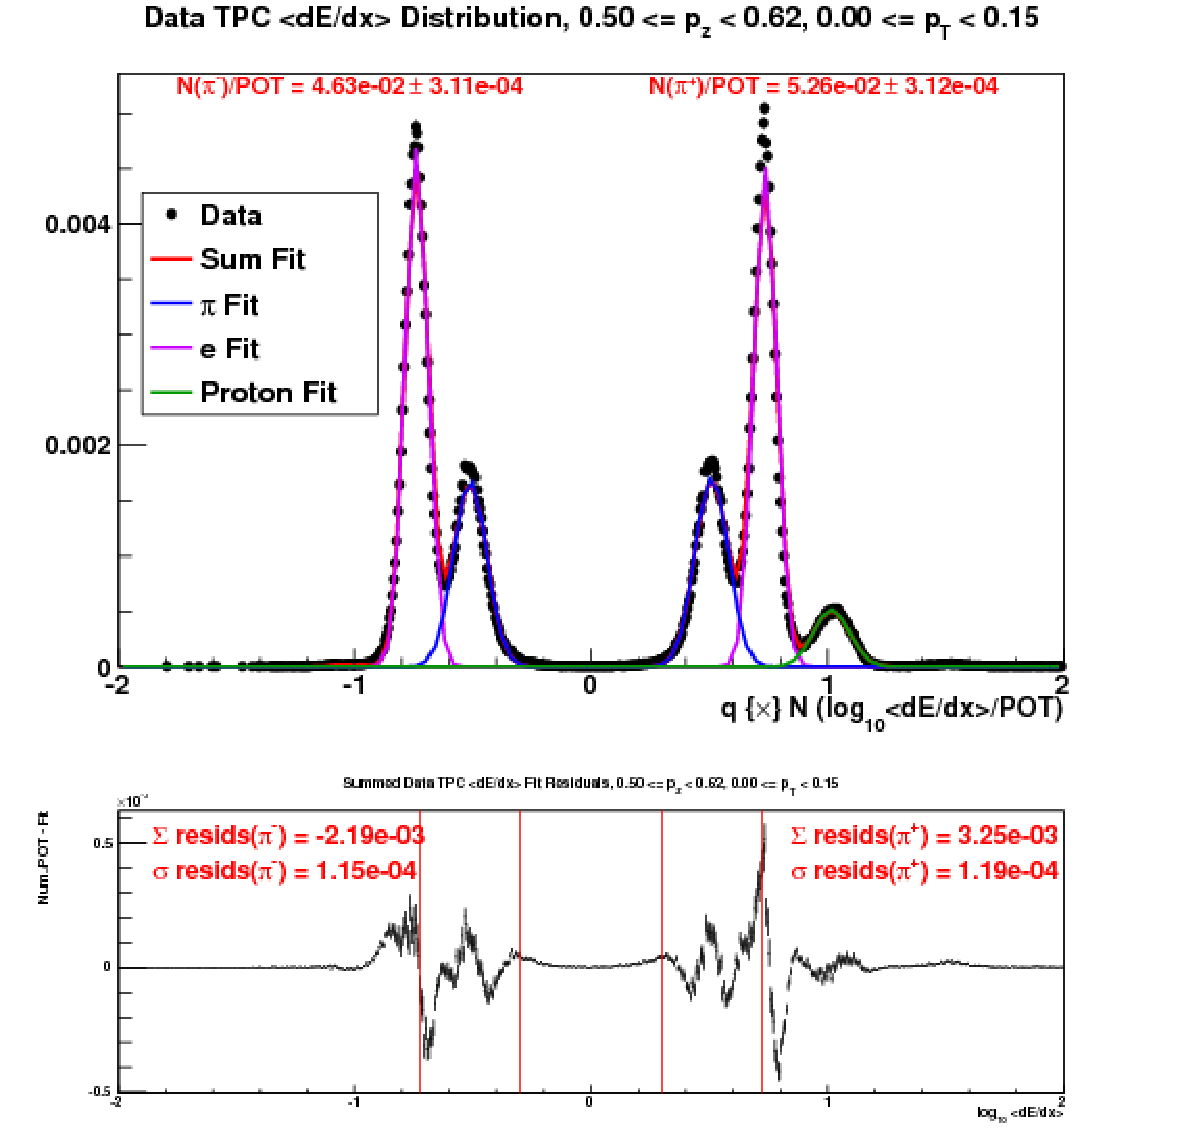
\includegraphics[width=0.45\textwidth]{fitdedx_data_4} 
   \caption{\dedx fit result for $0.5 \le p_z < 0.62, 0.0 \le p_T < 0.15$ GeV/c.}
   \label{fig:fitdedx4}
\end{figure}

\begin{figure}[!ht] %  figure placement: here, top, bottom, or page
   \centering
   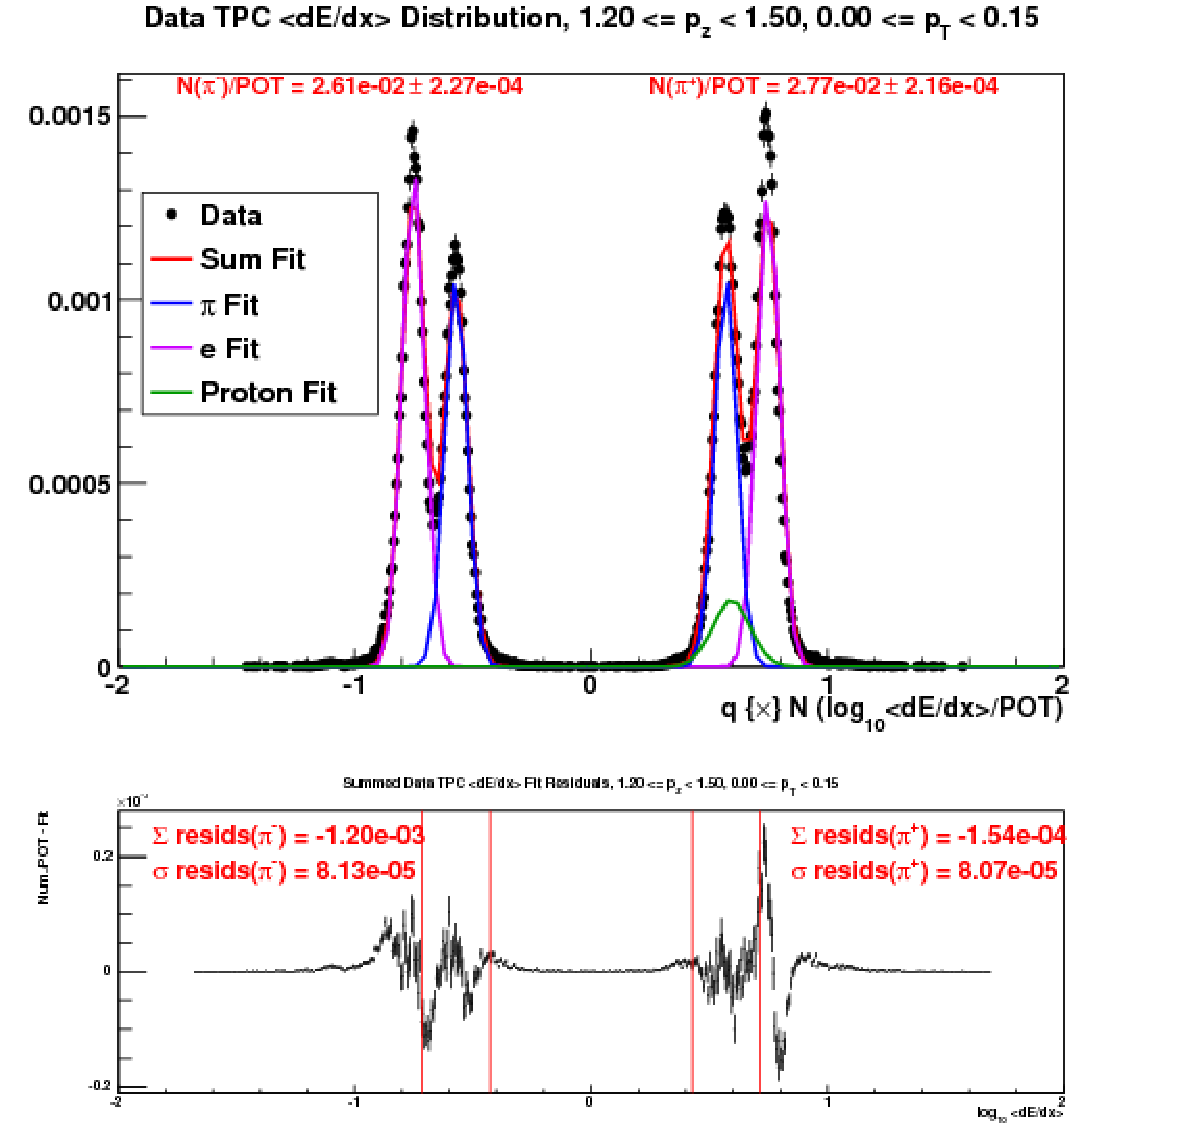
\includegraphics[width=0.45\textwidth]{fitdedx_data_24} 
   \caption{\dedx fit result for $1.2 \le p_z < 1.5, 0.0 \le p_T < 0.15$ GeV/c.}
   \label{fig:fitdedx24}
\end{figure}

Figs.~\ref{fig:fitdedx4} and \ref{fig:fitdedx24} show two examples of fits to the \dedx distributions for two bins, the former at lower momentum where the proton peak is clearly visible, and the latter at higher momentm where the proton peak falls mostly under the pion peak.  In the latter case, the green curve is constrained from the ToF data as described above.  

The initial pion yield in each \pzpt bin is taken as the sum of the integrals of the fitted pion Gaussian peaks for the two independent data sets where clean ToF data are used, and where only TPC data are used.  The uncertainty on the pion yield in each case is taken from the uncertainty in the fit parameters for the amplitude and width.  However, it is clear that these fits are not perfect, and the bottoms of Figs.~\ref{fig:fitdedx4} and \ref{fig:fitdedx24} show, the residuals of the fit (data - fit).  We take into account the imperfection of the fit by adding the sum of the residuals in the range $[-3\sigma,3\sigma]$ (the red lines in the Figures), where $\sigma$ is the fitted width of the Gaussian peak from the \emph{full} fit function, and the RMS of the residuals in these regions is taken as the uncertainty on this correction to the pion yield.  These corrections are typically on the order of 10\%, with typical uncertainties on the order of 10\%.  All uncertainties are added in quadrature.

\subsubsection{RICH Measurements}
\begin{figure}[!htb] %  figure placement: here, top, bottom, or page
   \centering
   \subfigure[$6.0 \le p_z < 8.0, 0.0 \le p_T < 0.15$ GeV/c, $q < 0$.]{\label{fig:rich_count_minus_44}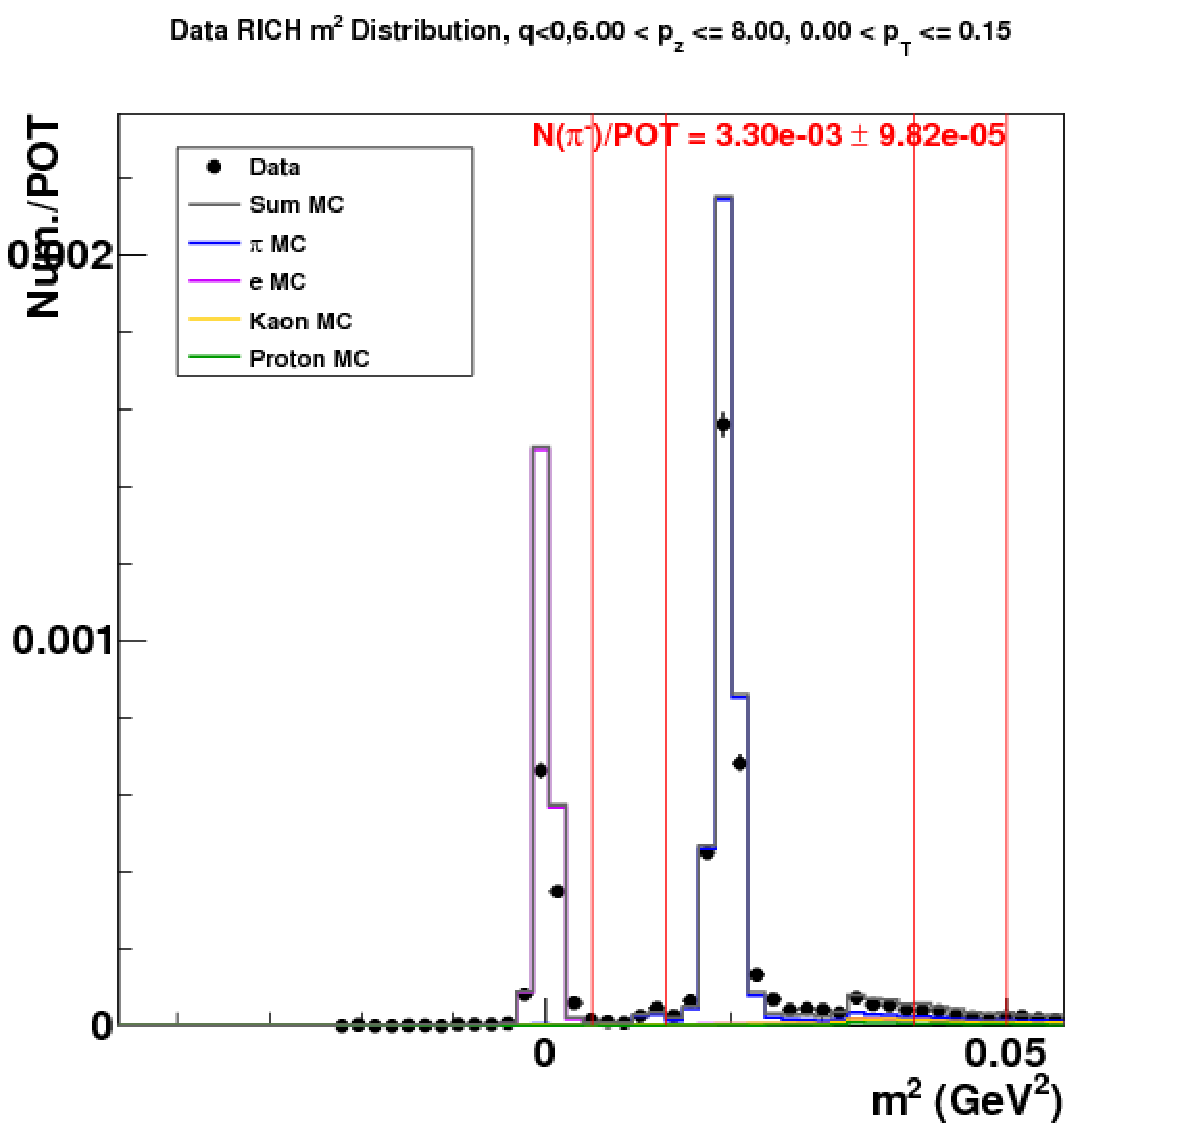
\includegraphics[width=0.45\textwidth]{rich_count_minus_44}} 
   \subfigure[$10.0 \le p_z < 14.0, 0.25 \le p_T < 0.45$ GeV/c, $q < 0$.]{\label{fig:rich_count_minus_54}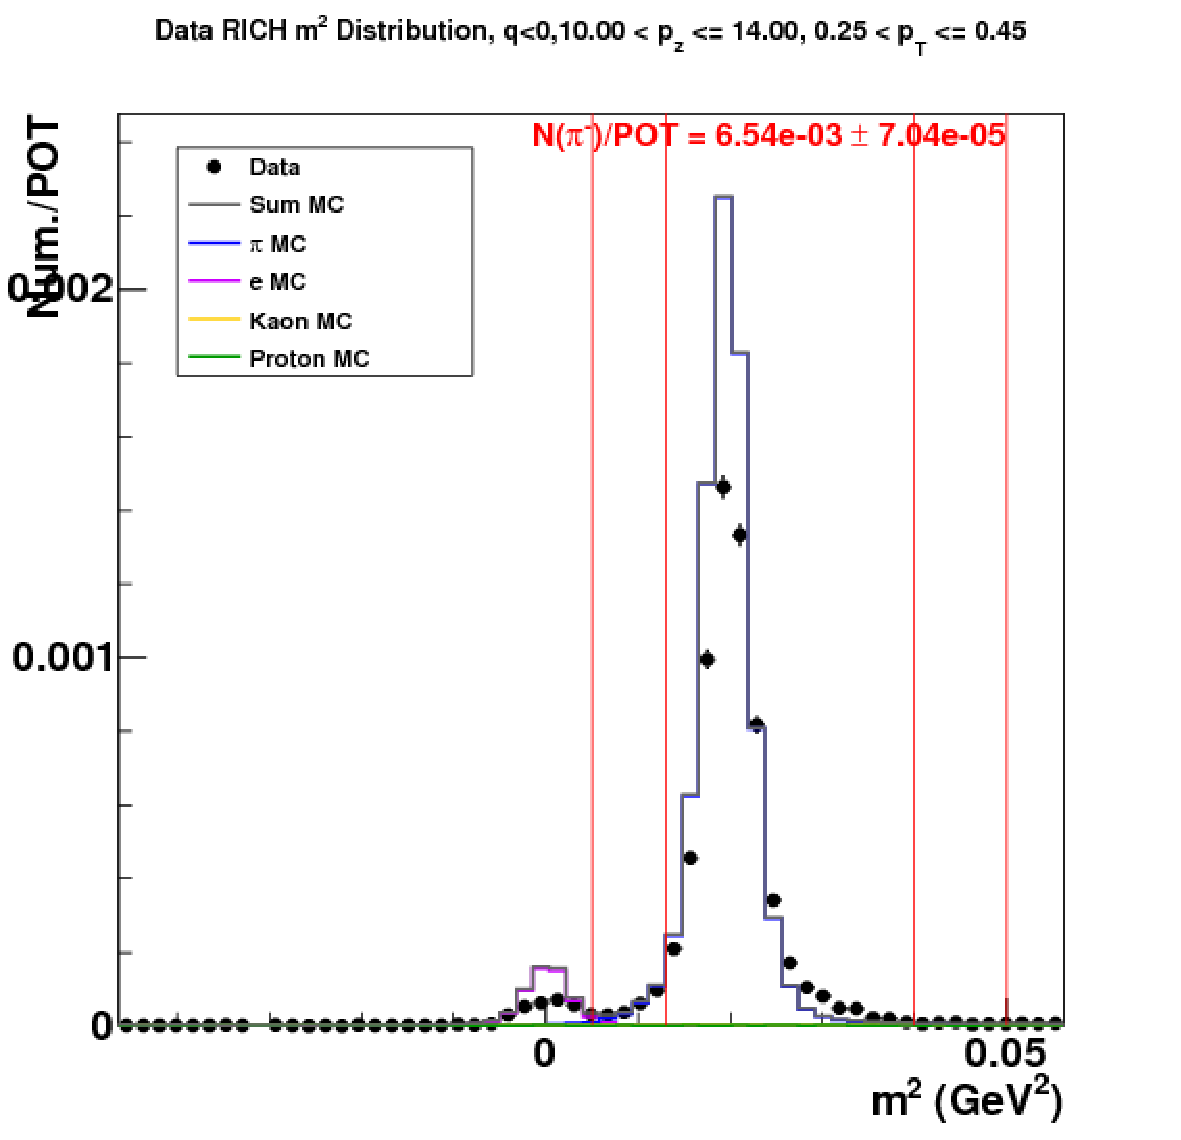
\includegraphics[width=0.45\textwidth]{rich_count_minus_54}}%
   \caption{RICH $m^2$ distributions, data (black dots) vs. MC (solid lines).  The solid vertical red lines represent the bounds to define the signal and side-band windows for background estimation.}
   \label{fig:richm2A}
\end{figure}
   
Given a particle's momentum, the matched RICH ring radius may be converted to a $m^2$ invariant assuming the small-angle approximation:
\begin{equation}
m^2 \simeq p^2 n^2\left(1 - \left(\frac{r}{L}\right)^2\right) - p^2
\end{equation}
where $n$ is the refractive index ($\sim1.00045$ for the CO$_2$ used in the MIPP RICH detector), $r$ is the reconstructed RICH ring radius and $L$ is the length of the RICH radiator volume (990 cm).
%The MC response of the RICH detector was tuned to calibrated data such that the peak positions in the $m^2$ distributions were flat as a function over momentum.  
The RICH $m^2$ distributions are not well described by Gaussians, however, in general, the $e, \pi, K$ and $p$ peaks in these distributions are quite well separated.  Therefore we take a simple cut-and-count approach, where we simply count the number of tracks that fall within a range in $m^2$ that contains pions.  In practice, however, there is contamination from non-pions, mostly electron/positrons, and a low-side tail of pions that sits under the electron peak that must be taken into account.  We assume that the shapes of the MC distributions for each particle are well described.  We then define three ranges, one main signal range and two side-band ranges in which we use the data to normalize the MC distributions in the sidebands.  Defining $N_i$ as the number of tracks within a range, $\bar{N}_i$ as the number of tracks inside the other two windows, $B_i$ as the MC background (number of non-pions) and $\bar{S}_i$ [$\bar{B}_i$] as the MC signal [background] outside the window, the pion yield is then:

\begin{equation}
N(\pi) = \sum_i N(\pi)_i,
\end{equation}

where $i$ is one of the three ranges and

\begin{equation}
N(\pi)_i = N_i^\mathrm{Data} - b_i^\mathrm{MC}\bar{N}_i^\mathrm{Data},
\end{equation}

\begin{equation}
b_i = \frac{B_i}{\bar{S}_i + \bar{B}_i}
\end{equation}

The uncertainty on the number of pions is

\begin{equation}
\sigma^2_{N(\pi)} = \sum_i \sigma^2_{N(\pi)_i}
\end{equation}

where 
\begin{equation}
\sigma^2_{N(\pi)_i} = N_i + \bar{N}_ib_i^2\left(1 + \bar{N}_i\left(\frac{\delta b_i}{b_i}\right)^2\right)
\end{equation}
$b_i$ represents the relative amounts of pion to non-pion background in each range in the MC, and we assume  a 30\% conservative systematic uncertainty in this ratio; the MC statistical uncertainty is negligible.  The positions and widths of the signal and side-band ranges are set by hand based on a visual scan of the $m^2$ distribution in each bin.  In some cases, the low-side range boundary cuts off some signal predicted by the MC; this is corrected  by determining the fraction of signal lost in this region in the MC and scaling by the measured $N(\pi)$ from data.
and a 30\% uncertainty is added to this correction.  Fig.~\ref{fig:richm2A} shows examples of data and MC RICH $m^2$ distributions; the window boundaries are defined by the vertical solid red lines, and the pion yield and uncertainty is displayed near the top of each in red.  In most cases the RICH pion yield has uncertainties of $\sim 5\%$.  

%\begin{equation}
%N(\pi)_\mathrm{corr} = N(\pi)\frac{\int_{-0.5}^\mathrm{lower-edge}N^\mathrm{MC}}{\int_\mathrm{lower-edge}^\mathrm{upper-edge}N^\mathrm{MC}}
%\end{equation}
\subsection{Statistical and Background Systematic Uncertainties}

The methods to determine the pion yields discussed above provide an 
uncertainty which combines statistical uncertainties and systematic uncertainties from backgrounds.  The relative 
uncertainties as a function of \pzpt are shown in Fig.~\ref{StatSystUncertaintyPos} for the $\pi^+$ yields; the uncertainties are similar for the $\pi^-$ yields.  In general, the combined uncertainty is a few percent for most bins of \pzpt where a measurement is made; the colorless bins are those with no measurement.

\begin{figure}[!ht] %  figure placement: here, top, bottom, or page
   \centering
   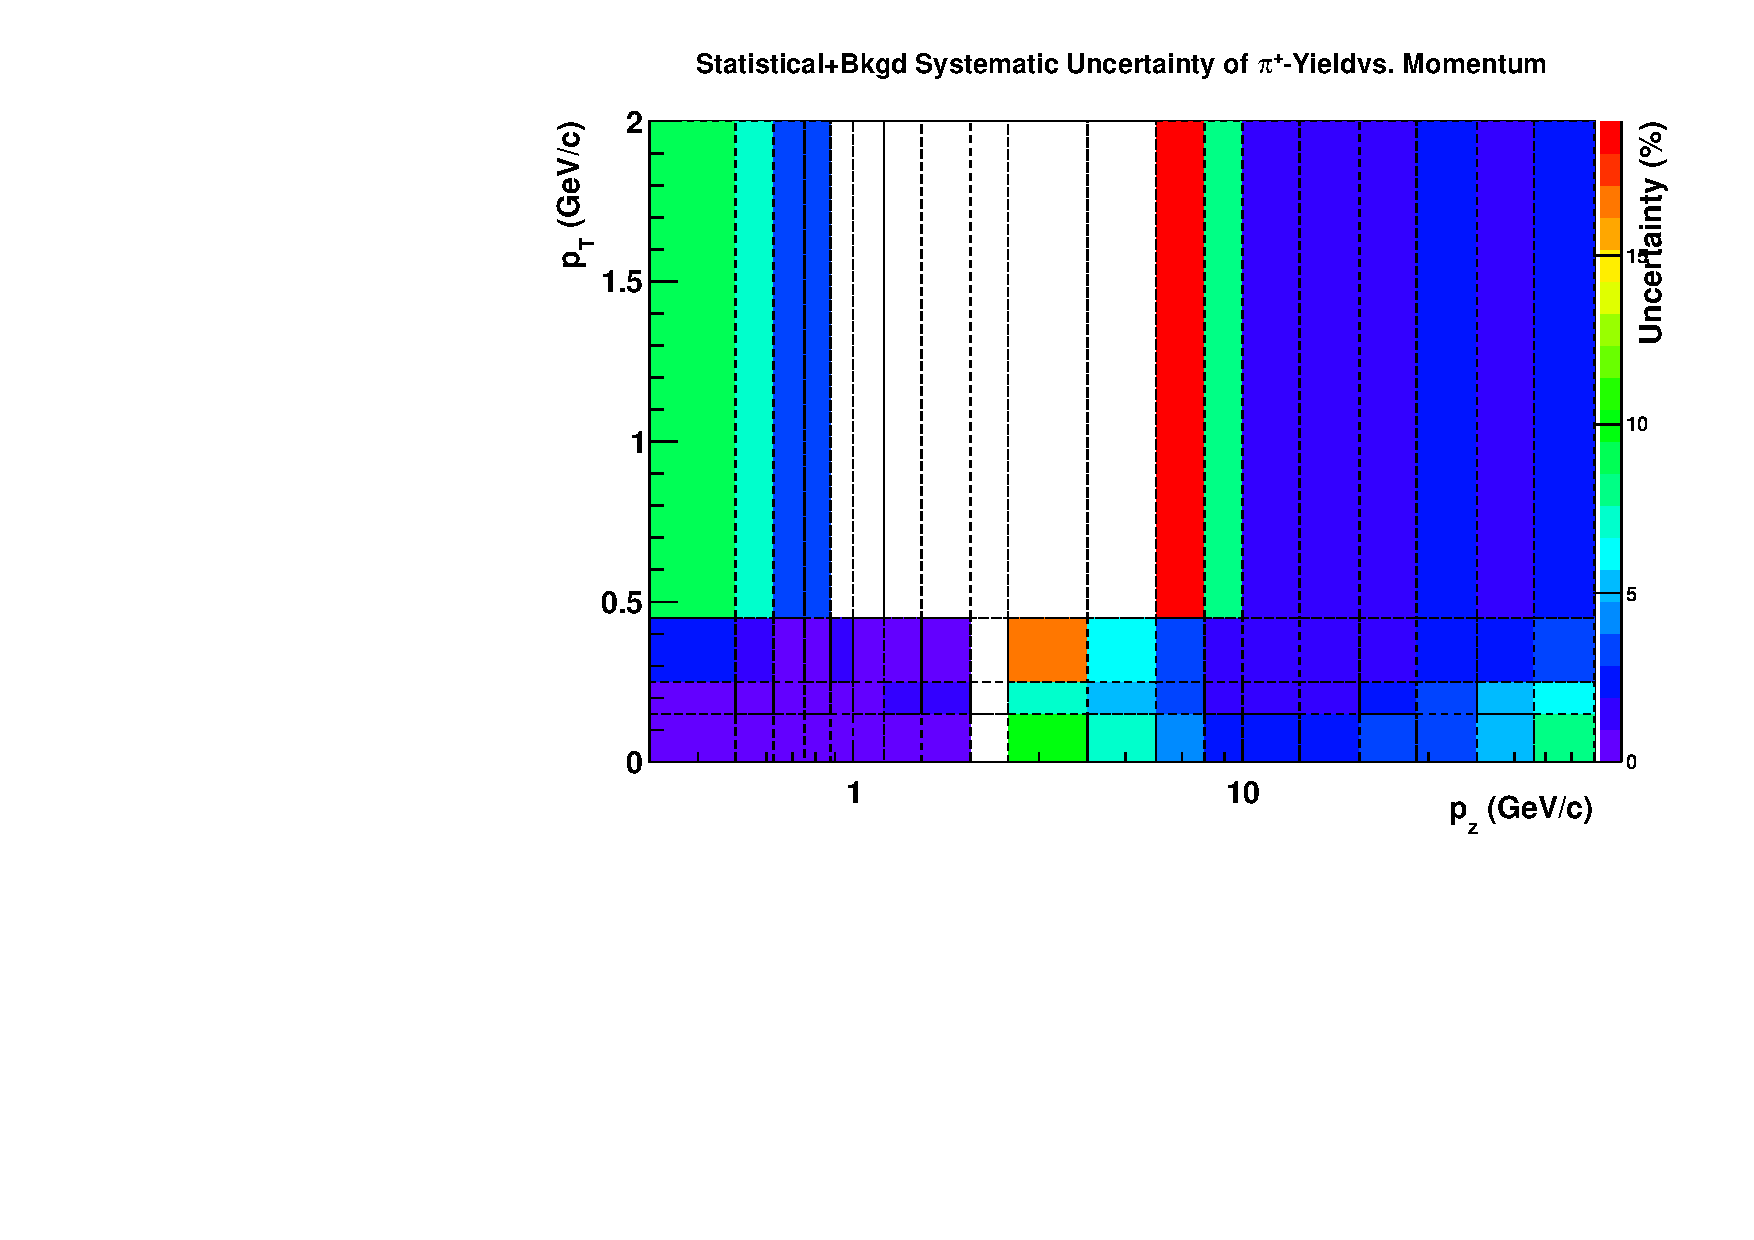
\includegraphics[width=0.45\textwidth]{StatSystUncertaintyPos} 
   \caption{Combined statistical and background systematic uncertainties of the $\pi^+$ yields as a function of \pzpt.  The colors on the z-axis represent the fractional uncertainty of each measurement.}
   \label{fig:StatSyst}
\end{figure}

\subsection{Systematic Uncertainties}

The uncertainty of the acceptance and efficiency corrections that are applied to the measured yields in each bin arises from MC statistics ($\sim 8\times$ that of data), imperfections in the geometry model of the spectrometer (negligible), imperfections in the modeling of the performance of the tracking and PID detectors, and incorrect modeling of the particle yields in the MC.  

The time-dependency of channel masks and thresholds used in the data collection, reconstruction and analysis was also used in the generation, reconstruction and analysis of the MC.  The time-dependent masks and thresholds are known to within a few percent in each run.  We therefore assume a 2\% uncertainty on all efficiencies due to imperfections in the modeling of the detectors in the MC.

Incorrect modeling of the particle yields in the MC results in improper modeling of pileup of secondary particles off the target.  Pileup is the main cause of reconstruction and PID inefficiency.  To correct for this, MC events are reweighted such that the multiplicity distribution (number of charged tracks coming off the surface of the target) in MC matches that of data, and the efficiencies are re-calculated.  The difference between the nominal and the reweighted MC is taken as the systematic uncertainty due to this effect.  

\subsection{Results}

The measured $N(\pi^+)$/POT and $N(\pi^-)$/POT per \pzpt bin, along with the combined statistical and systematic errors, are shown in Fig.~\ref{fig:FinalYields} and Tables \ref{table:FinalPiPlusYields} and \ref{table:FinalPiMinusYields}.  The uncertainties in the table are fractional, in units of percent.  We see that in most of the bins, the measurements are systematics limited, even at higher momenta, and nearly all measurements have uncertainties estimated below 10\%.  Fig.~\ref{fig:FinalRatios} shows the ratio, $R$, of
 $\pi^-/\pi^+$ yields as a function of $p_z$ in slices of $p_T$.  Table \ref{table:FinalPiRatios} lists the $R$-values measured in each bin along with the statistical and systematic uncertainties.  Correlated systematics between the positive and negative pion yields have been subtracted out in the ratios by assuming $\delta R(\pi)^2_\mathrm{syst} = |\delta N(\pi^+)^2 - \delta N(\pi^-)^2|$.

\begin{figure}[!t] %  figure placement: here, top, bottom, or page
   \centering
   \subfigure[Measured $N(\pi^+)$/POT.]{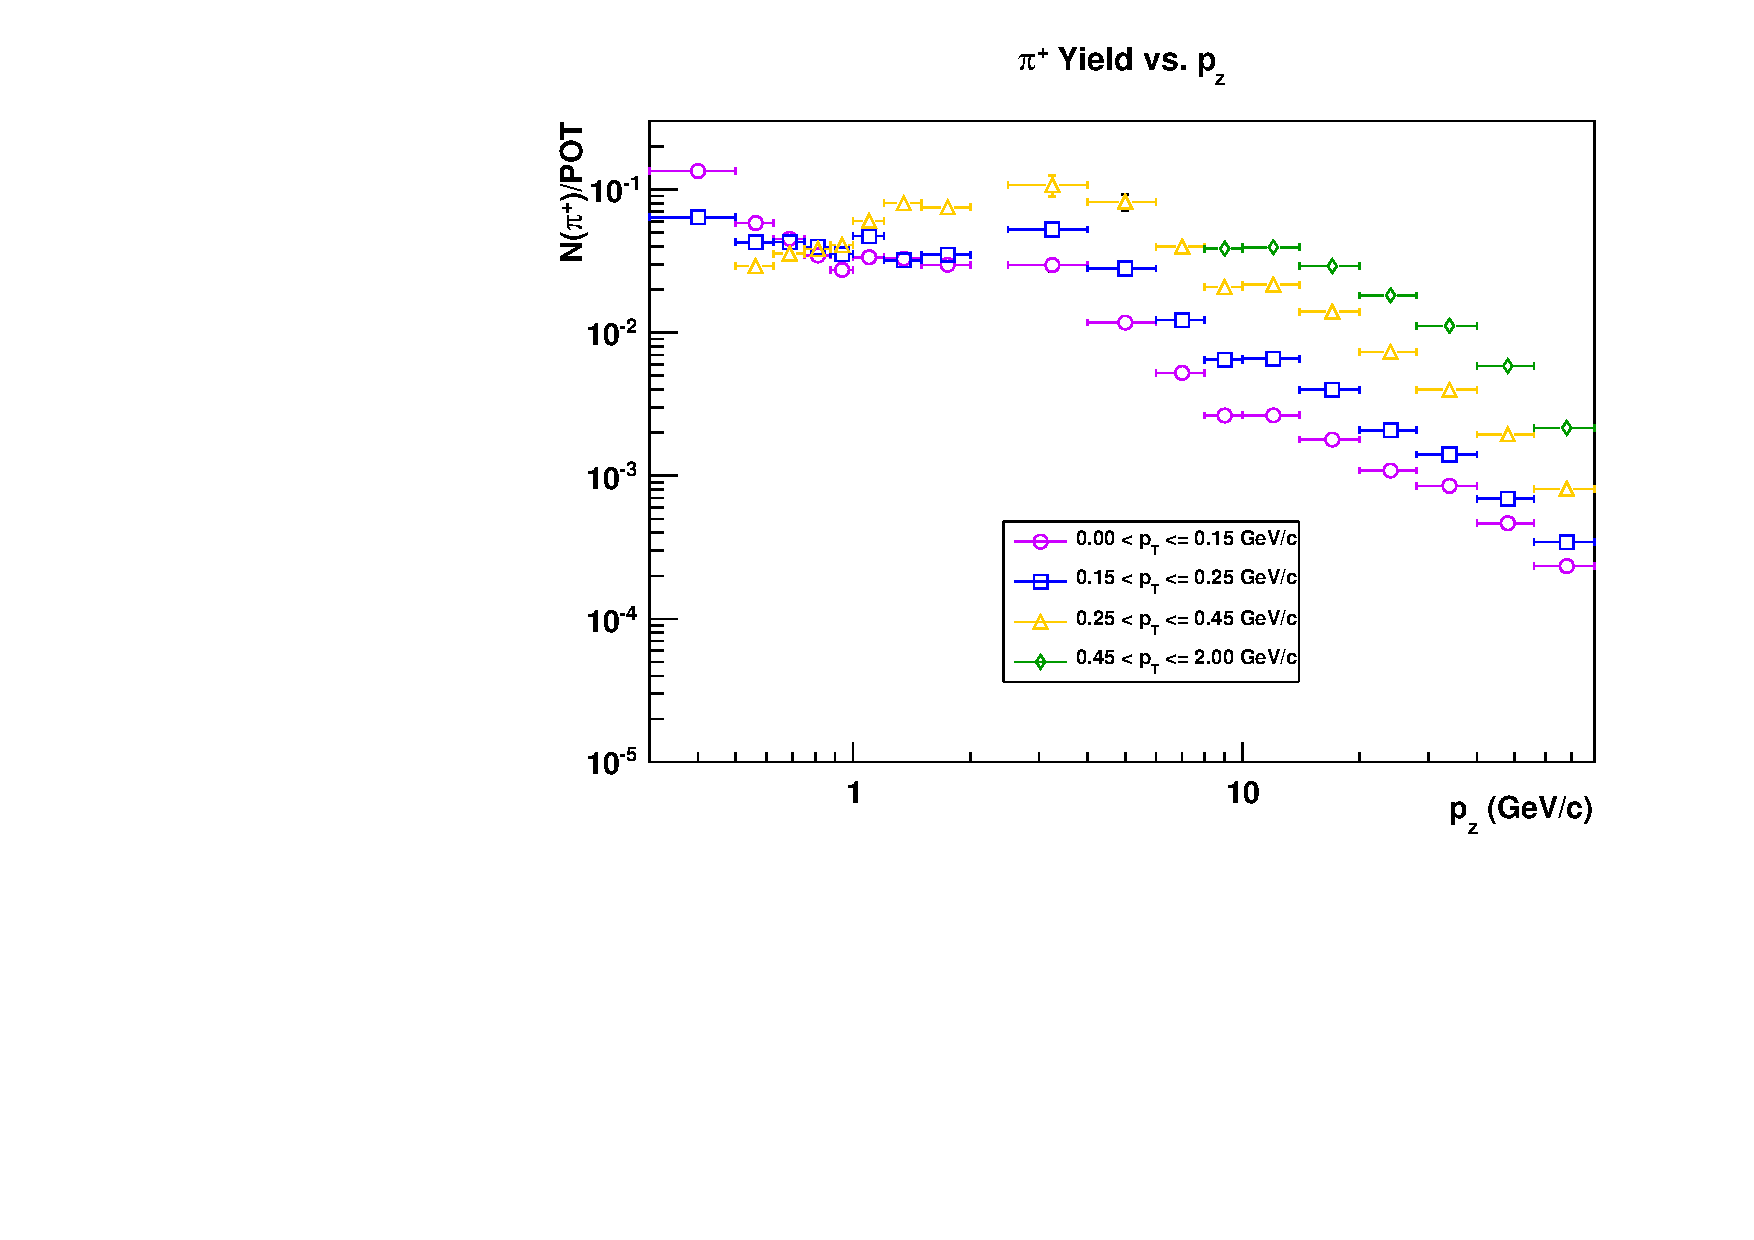
\includegraphics[width=0.48\textwidth]{hPi1D_plus}}  
   \subfigure[Measured $N(\pi^-)$/POT.]{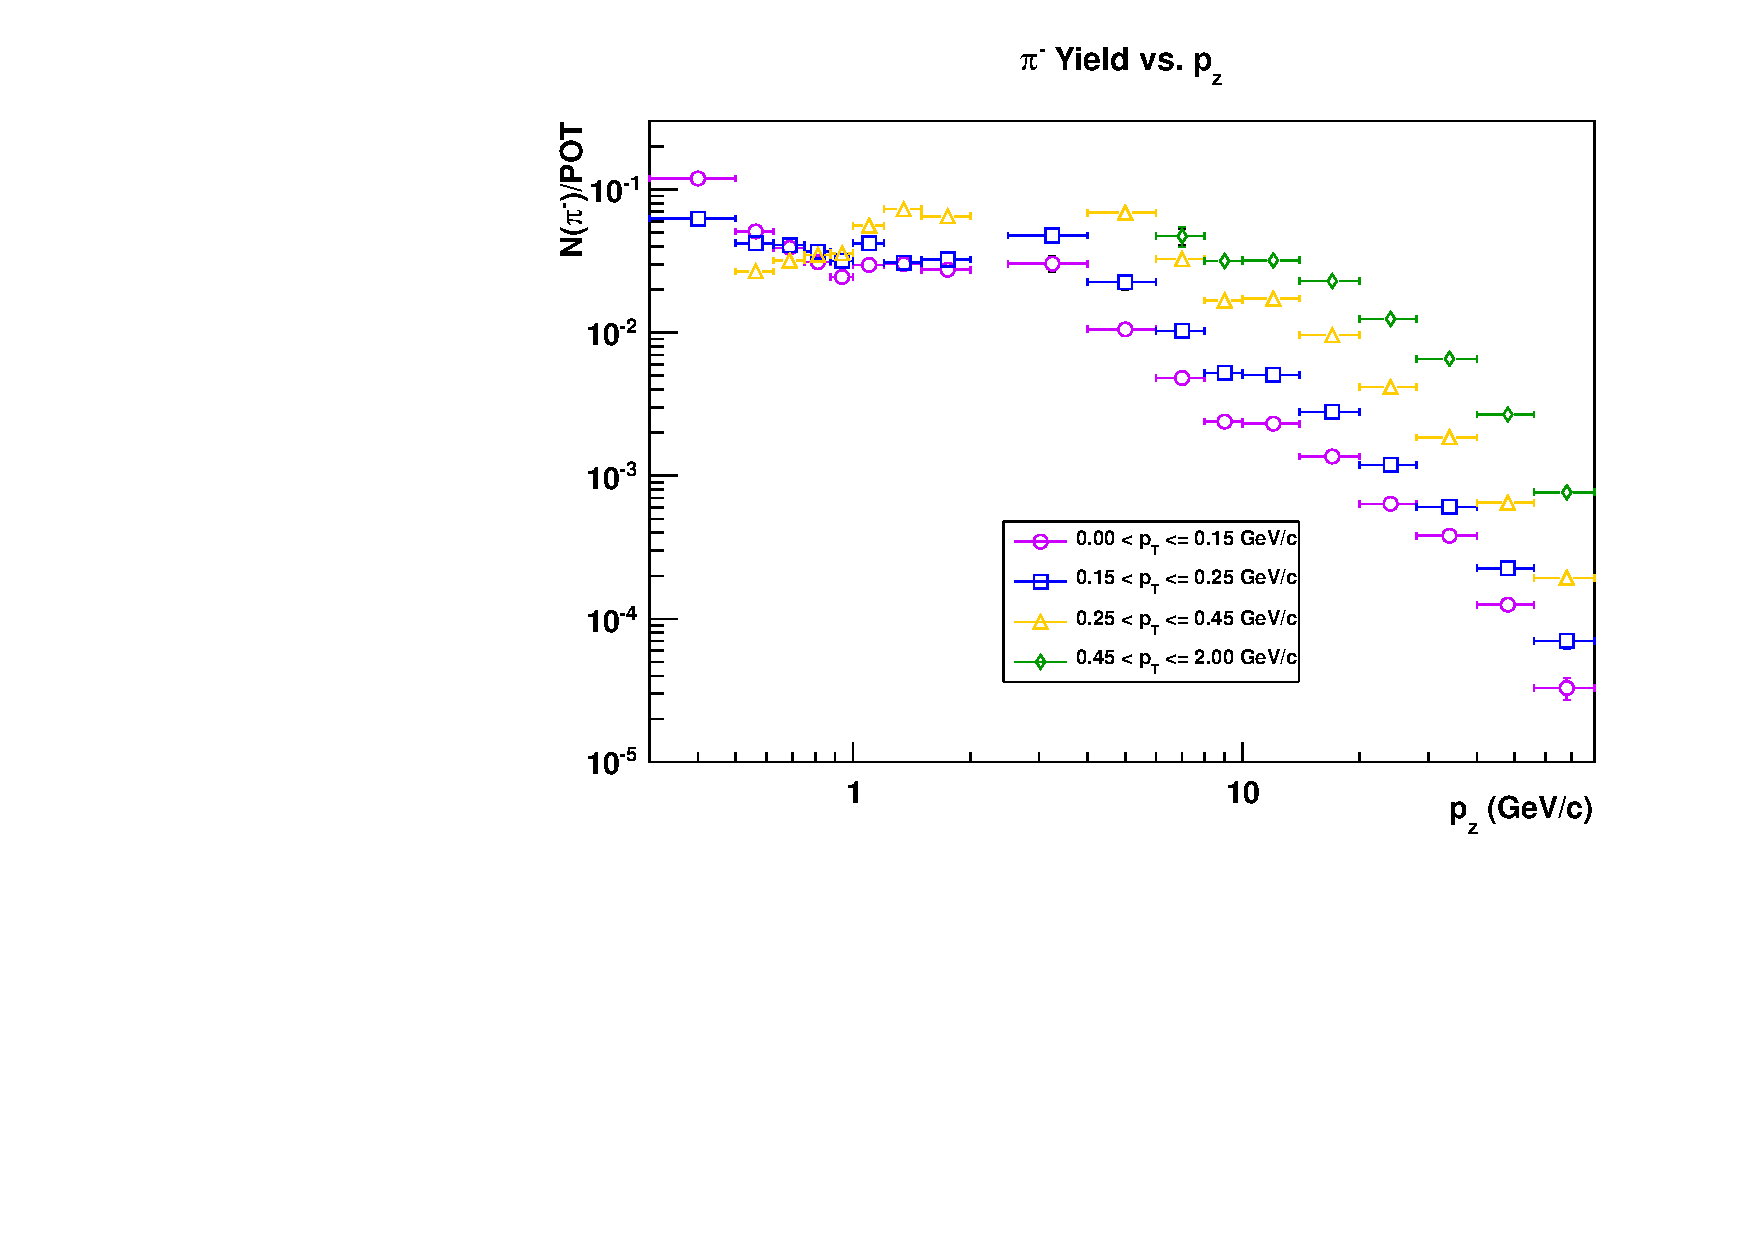
\includegraphics[width=0.48\textwidth]{hPi1D_minus}}%   
   \caption{Final pion yields as a function of $p_z$ in bins of $p_T$ (different colors and markers represent bins of $p_T$.  All efficiency corrections have been applied, and both statistical and systematic error bars are plotted.}
   \label{fig:FinalYields}
\end{figure}

\begin{figure}[!htbp] %  figure placement: here, top, bottom, or page
   \centering
   \subfigure[ $R_{\mathrm{Data}}(\pi)$]{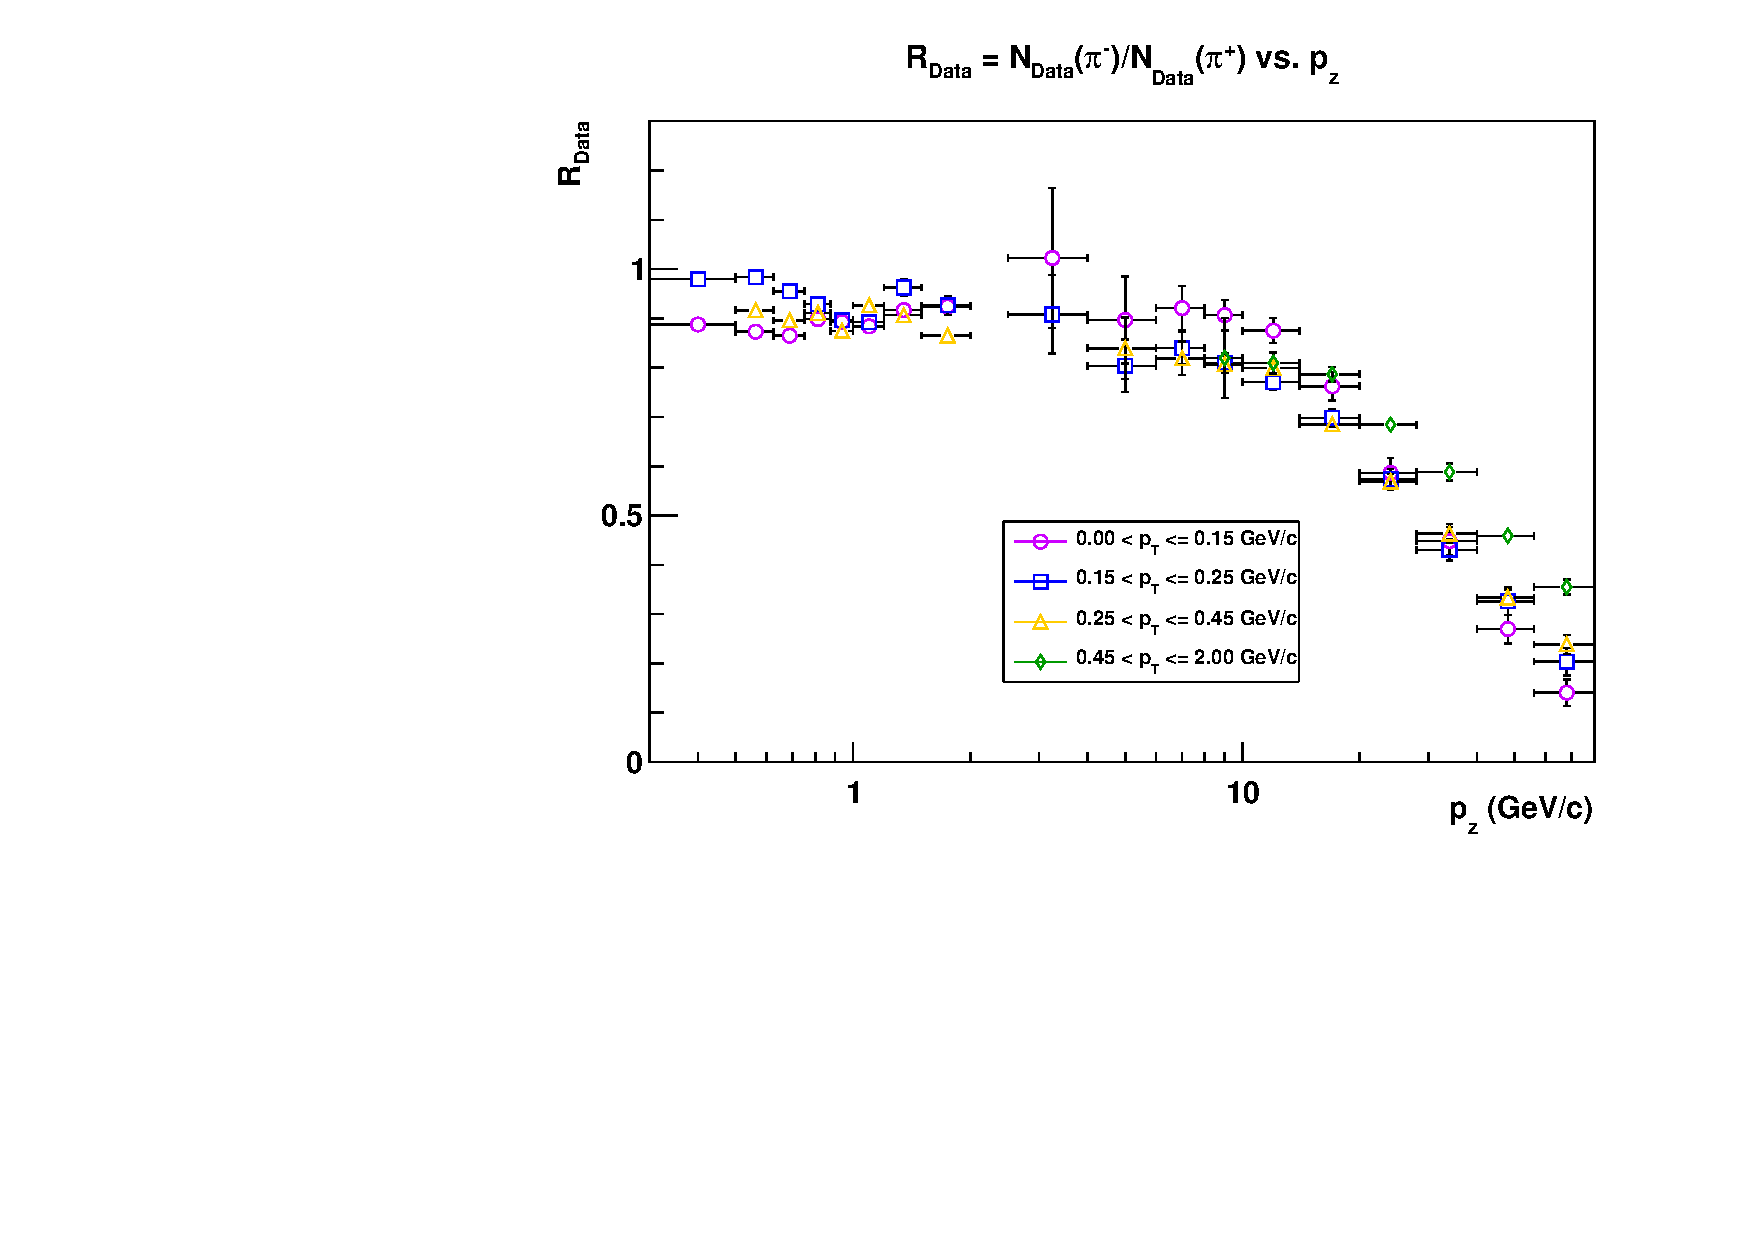
\includegraphics[width=0.48\textwidth]{hPiRatio1D}}  
   \caption{Final charge pion yield ratios as a function of $p_z$ in bins of $p_T$ (different colors and markers represent bins of $p_T$.  All efficiency corrections have been applied, and both statistical and systematic error bars are plotted.}
   \label{fig:FinalRatios}
\end{figure}

\begin{table}
\caption{NuMI target $\pi^+$ Yield}
\begin{tabular}{|c|c|c|c|c|}
\hline
\textbf{$p_z$} & \textbf{$p_T$} & \textbf{$N(\pi^+)/$} & \textbf{stat+} & \textbf{syst}\\
\textbf{(GeV/c)} &\textbf{(GeV/c)} & \textbf{POT}& \textbf{bkgd}& \textbf{(\%)}\\
& & & \textbf{(\%)} & \\
\hline

[0.30,0.50) & [0.00,0.15) & 1.34e-01 & 0.50 & 4.60 \\ 
 \hline
[0.30,0.50) & [0.15,0.25) & 6.39e-02 & 0.68 & 7.07 \\ 
 \hline
[0.50,0.62) & [0.00,0.15) & 5.83e-02 & 0.59 & 4.34 \\ 
 \hline
[0.50,0.62) & [0.15,0.25) & 4.28e-02 & 0.70 & 4.81 \\ 
 \hline
[0.50,0.62) & [0.25,0.45) & 2.92e-02 & 1.03 & 7.66 \\ 
 \hline
[0.62,0.75) & [0.00,0.15) & 4.52e-02 & 0.66 & 4.40 \\ 
 \hline
[0.62,0.75) & [0.15,0.25) & 4.28e-02 & 0.66 & 4.71 \\ 
 \hline
[0.62,0.75) & [0.25,0.45) & 3.56e-02 & 0.81 & 6.49 \\ 
 \hline
[0.75,0.88) & [0.00,0.15) & 3.46e-02 & 0.81 & 4.52 \\ 
 \hline
[0.75,0.88) & [0.15,0.25) & 3.96e-02 & 0.67 & 4.33 \\ 
 \hline
[0.75,0.88) & [0.25,0.45) & 3.84e-02 & 0.74 & 5.10 \\ 
 \hline
[0.88,1.00) & [0.00,0.15) & 2.74e-02 & 0.82 & 4.72 \\ 
 \hline
[0.88,1.00) & [0.15,0.25) & 3.54e-02 & 0.71 & 4.15 \\ 
 \hline
[0.88,1.00) & [0.25,0.45) & 4.09e-02 & 1.01 & 5.12 \\ 
 \hline
[1.00,1.20) & [0.00,0.15) & 3.36e-02 & 0.78 & 4.57 \\ 
 \hline
[1.00,1.20) & [0.15,0.25) & 4.72e-02 & 0.67 & 4.38 \\ 
 \hline
[1.00,1.20) & [0.25,0.45) & 6.04e-02 & 0.74 & 4.57 \\ 
 \hline
[1.20,1.50) & [0.00,0.15) & 3.29e-02 & 0.78 & 4.63 \\ 
 \hline
[1.20,1.50) & [0.15,0.25) & 3.20e-02 & 1.42 & 5.38 \\ 
 \hline
[1.20,1.50) & [0.25,0.45) & 8.03e-02 & 0.51 & 4.56 \\ 
 \hline
[1.50,2.00) & [0.00,0.15) & 2.98e-02 & 0.89 & 4.30 \\ 
 \hline
[1.50,2.00) & [0.15,0.25) & 3.50e-02 & 1.80 & 5.44 \\ 
 \hline
[1.50,2.00) & [0.25,0.45) & 7.51e-02 & 0.90 & 4.80 \\ 
 \hline
[2.50,4.00) & [0.00,0.15) & 2.96e-02 & 9.71 & 10.37 \\ 
 \hline
[2.50,4.00) & [0.15,0.25) & 5.26e-02 & 7.41 & 7.28 \\ 
 \hline
[2.50,4.00) & [0.25,0.45) & 1.07e-01 & 16.48 & 6.59 \\ 
 \hline
[4.00,6.00) & [0.00,0.15) & 1.17e-02 & 7.21 & 5.18 \\ 
 \hline
[4.00,6.00) & [0.15,0.25) & 2.81e-02 & 5.24 & 5.03 \\ 
 \hline
[4.00,6.00) & [0.25,0.45) & 8.20e-02 & 6.42 & 12.66 \\ 
 \hline
[6.00,8.00) & [0.00,0.15) & 5.24e-03 & 3.92 & 4.81 \\ 
 \hline
[6.00,8.00) & [0.15,0.25) & 1.22e-02 & 3.17 & 4.63 \\ 
 \hline
[6.00,8.00) & [0.25,0.45) & 3.99e-02 & 3.43 & 4.35 \\ 
 \hline
[8.00,10.00) & [0.00,0.15) & 2.64e-03 & 2.54 & 5.35 \\ 
 \hline
[8.00,10.00) & [0.15,0.25) & 6.46e-03 & 1.79 & 4.65 \\ 
 \hline
[8.00,10.00) & [0.25,0.45) & 2.08e-02 & 1.50 & 4.95 \\ 
 \hline
[8.00,10.00) & [0.45,2.00) & 3.86e-02 & 8.44 & 10.21 \\ 
 \hline
[10.00,14.00) & [0.00,0.15) & 2.64e-03 & 2.01 & 4.53 \\ 
 \hline
[10.00,14.00) & [0.15,0.25) & 6.58e-03 & 1.36 & 3.84 \\ 
 \hline
[10.00,14.00) & [0.25,0.45) & 2.16e-02 & 1.04 & 4.49 \\ 
 \hline
[10.00,14.00) & [0.45,2.00) & 3.95e-02 & 1.79 & 8.52 \\ 
 \hline
[14.00,20.00) & [0.00,0.15) & 1.79e-03 & 2.46 & 5.37 \\ 
 \hline
[14.00,20.00) & [0.15,0.25) & 4.00e-03 & 1.63 & 4.87 \\ 
 \hline
[14.00,20.00) & [0.25,0.45) & 1.40e-02 & 1.04 & 4.32 \\ 
 \hline
[14.00,20.00) & [0.45,2.00) & 2.91e-02 & 1.26 & 4.52 \\ 
 \hline
[20.00,28.00) & [0.00,0.15) & 1.09e-03 & 3.15 & 6.38 \\ 
 \hline
[20.00,28.00) & [0.15,0.25) & 2.08e-03 & 2.22 & 4.27 \\ 
 \hline
[20.00,28.00) & [0.25,0.45) & 7.34e-03 & 1.60 & 4.59 \\ 
 \hline
[20.00,28.00) & [0.45,2.00) & 1.82e-02 & 1.29 & 4.51 \\ 
 \hline
[28.00,40.00) & [0.00,0.15) & 8.50e-04 & 3.52 & 4.92 \\ 
 \hline
[28.00,40.00) & [0.15,0.25) & 1.41e-03 & 2.88 & 5.55 \\ 
 \hline
[28.00,40.00) & [0.25,0.45) & 4.00e-03 & 2.31 & 3.71 \\ 
 \hline
[28.00,40.00) & [0.45,2.00) & 1.12e-02 & 2.15 & 4.54 \\ 
 \hline
[40.00,56.00) & [0.00,0.15) & 4.66e-04 & 5.64 & 5.34 \\ 
 \hline
[40.00,56.00) & [0.15,0.25) & 6.91e-04 & 5.34 & 5.31 \\ 
 \hline
[40.00,56.00) & [0.25,0.45) & 1.94e-03 & 2.27 & 3.71 \\ 
 \hline
[40.00,56.00) & [0.45,2.00) & 5.84e-03 & 1.44 & 4.64 \\ 
 \hline
[56.00,80.00) & [0.00,0.15) & 2.34e-04 & 7.79 & 7.12 \\ 
 \hline
[56.00,80.00) & [0.15,0.25) & 3.44e-04 & 6.54 & 3.88 \\ 
 \hline
[56.00,80.00) & [0.25,0.45) & 8.10e-04 & 3.71 & 4.58 \\ 
 \hline
[56.00,80.00) & [0.45,2.00) & 2.16e-03 & 2.36 & 4.06 \\ 
 \hline
\end{tabular}
\label{table:FinalPiPlusYields}
\end{table}

\begin{table}
\caption{NuMI target $\pi^-$ Yield}
\begin{tabular}{|c|c|c|c|c|}
\hline

\textbf{$p_z$} & \textbf{$p_T$} & \textbf{$N(\pi^+)/$} & \textbf{stat+} & \textbf{syst}\\
\textbf{(GeV/c)} &\textbf{(GeV/c)} & \textbf{POT}& \textbf{bkgd}& \textbf{(\%)}\\
& & & \textbf{(\%)} & \\

\hline

[0.30,0.50) & [0.00,0.15) & 1.19e-01 & 0.53 & 5.29 \\ 
 \hline
[0.30,0.50) & [0.15,0.25) & 6.26e-02 & 0.68 & 7.37 \\ 
 \hline
[0.50,0.62) & [0.00,0.15) & 5.09e-02 & 0.67 & 5.10 \\ 
 \hline
[0.50,0.62) & [0.15,0.25) & 4.21e-02 & 0.69 & 5.74 \\ 
 \hline
[0.50,0.62) & [0.25,0.45) & 2.68e-02 & 0.99 & 8.01 \\ 
 \hline
[0.62,0.75) & [0.00,0.15) & 3.91e-02 & 0.75 & 5.12 \\ 
 \hline
[0.62,0.75) & [0.15,0.25) & 4.09e-02 & 0.69 & 5.48 \\ 
 \hline
[0.62,0.75) & [0.25,0.45) & 3.19e-02 & 0.84 & 7.31 \\ 
 \hline
[0.75,0.88) & [0.00,0.15) & 3.11e-02 & 0.85 & 5.20 \\ 
 \hline
[0.75,0.88) & [0.15,0.25) & 3.68e-02 & 0.70 & 5.32 \\ 
 \hline
[0.75,0.88) & [0.25,0.45) & 3.50e-02 & 0.76 & 6.07 \\ 
 \hline
[0.88,1.00) & [0.00,0.15) & 2.45e-02 & 0.88 & 5.16 \\ 
 \hline
[0.88,1.00) & [0.15,0.25) & 3.17e-02 & 0.76 & 5.26 \\ 
 \hline
[0.88,1.00) & [0.25,0.45) & 3.58e-02 & 0.74 & 5.91 \\ 
 \hline
[1.00,1.20) & [0.00,0.15) & 2.97e-02 & 0.85 & 5.38 \\ 
 \hline
[1.00,1.20) & [0.15,0.25) & 4.21e-02 & 0.69 & 5.30 \\ 
 \hline
[1.00,1.20) & [0.25,0.45) & 5.59e-02 & 0.61 & 5.69 \\ 
 \hline
[1.20,1.50) & [0.00,0.15) & 3.01e-02 & 0.87 & 5.05 \\ 
 \hline
[1.20,1.50) & [0.15,0.25) & 3.08e-02 & 1.04 & 5.81 \\ 
 \hline
[1.20,1.50) & [0.25,0.45) & 7.28e-02 & 0.52 & 5.53 \\ 
 \hline
[1.50,2.00) & [0.00,0.15) & 2.75e-02 & 0.93 & 5.09 \\ 
 \hline
[1.50,2.00) & [0.15,0.25) & 3.25e-02 & 1.02 & 5.65 \\ 
 \hline
[1.50,2.00) & [0.25,0.45) & 6.50e-02 & 0.68 & 5.51 \\ 
 \hline
[2.50,4.00) & [0.00,0.15) & 3.03e-02 & 9.94 & 12.57 \\ 
 \hline
[2.50,4.00) & [0.15,0.25) & 4.77e-02 & 4.71 & 8.97 \\ 
 \hline
[4.00,6.00) & [0.00,0.15) & 1.05e-02 & 6.69 & 6.15 \\ 
 \hline
[4.00,6.00) & [0.15,0.25) & 2.25e-02 & 4.04 & 11.95 \\ 
 \hline
[4.00,6.00) & [0.25,0.45) & 6.88e-02 & 3.74 & 9.65 \\ 
 \hline
[6.00,8.00) & [0.00,0.15) & 4.82e-03 & 2.87 & 5.96 \\ 
 \hline
[6.00,8.00) & [0.15,0.25) & 1.03e-02 & 2.21 & 6.01 \\ 
 \hline
[6.00,8.00) & [0.25,0.45) & 3.27e-02 & 2.32 & 5.30 \\ 
 \hline
[6.00,8.00) & [0.45,2.00) & 4.72e-02 & 16.14 & 13.51 \\ 
 \hline
[8.00,10.00) & [0.00,0.15) & 2.39e-03 & 2.23 & 6.82 \\ 
 \hline
[8.00,10.00) & [0.15,0.25) & 5.23e-03 & 1.71 & 5.39 \\ 
 \hline
[8.00,10.00) & [0.25,0.45) & 1.68e-02 & 1.47 & 5.11 \\ 
 \hline
[8.00,10.00) & [0.45,2.00) & 3.16e-02 & 5.12 & 5.66 \\ 
 \hline
[10.00,14.00) & [0.00,0.15) & 2.31e-03 & 2.11 & 7.86 \\ 
 \hline
[10.00,14.00) & [0.15,0.25) & 5.07e-03 & 1.50 & 4.96 \\ 
 \hline
[10.00,14.00) & [0.25,0.45) & 1.73e-02 & 1.08 & 5.44 \\ 
 \hline
[10.00,14.00) & [0.45,2.00) & 3.20e-02 & 1.94 & 7.04 \\ 
 \hline
[14.00,20.00) & [0.00,0.15) & 1.36e-03 & 2.86 & 7.81 \\ 
 \hline
[14.00,20.00) & [0.15,0.25) & 2.79e-03 & 1.96 & 6.24 \\ 
 \hline
[14.00,20.00) & [0.25,0.45) & 9.60e-03 & 1.22 & 5.17 \\ 
 \hline
[14.00,20.00) & [0.45,2.00) & 2.29e-02 & 1.33 & 5.52 \\ 
 \hline
[20.00,28.00) & [0.00,0.15) & 6.37e-04 & 4.24 & 7.54 \\ 
 \hline
[20.00,28.00) & [0.15,0.25) & 1.19e-03 & 2.99 & 4.89 \\ 
 \hline
[20.00,28.00) & [0.25,0.45) & 4.18e-03 & 2.21 & 4.91 \\ 
 \hline
[20.00,28.00) & [0.45,2.00) & 1.25e-02 & 1.39 & 4.89 \\ 
 \hline
[28.00,40.00) & [0.00,0.15) & 3.81e-04 & 5.24 & 7.53 \\ 
 \hline
[28.00,40.00) & [0.15,0.25) & 6.05e-04 & 4.17 & 6.78 \\ 
 \hline
[28.00,40.00) & [0.25,0.45) & 1.85e-03 & 3.51 & 4.85 \\ 
 \hline
[28.00,40.00) & [0.45,2.00) & 6.56e-03 & 2.05 & 5.16 \\ 
 \hline
[40.00,56.00) & [0.00,0.15) & 1.26e-04 & 9.13 & 5.11 \\ 
 \hline
[40.00,56.00) & [0.15,0.25) & 2.25e-04 & 6.72 & 5.95 \\ 
 \hline
[40.00,56.00) & [0.25,0.45) & 6.49e-04 & 3.98 & 6.18 \\ 
 \hline
[40.00,56.00) & [0.45,2.00) & 2.68e-03 & 2.09 & 5.55 \\ 
 \hline
[56.00,80.00) & [0.00,0.15) & 3.29e-05 & 17.71 & 10.31 \\ 
 \hline
[56.00,80.00) & [0.15,0.25) & 7.01e-05 & 12.08 & 5.09 \\ 
 \hline
[56.00,80.00) & [0.25,0.45) & 1.93e-04 & 7.29 & 4.99 \\ 
 \hline
[56.00,80.00) & [0.45,2.00) & 7.67e-04 & 3.74 & 6.90 \\ 
 \hline
\end{tabular}
\label{table:FinalPiMinusYields}
\end{table}

\begin{table}
\caption{$\pi^-/\pi^+$ Ratio Production off NuMI target}
\begin{tabular}{|c|c|c|c|c|}
\hline

\textbf{$p_z$} & \textbf{$p_T$} & \textbf{$N(\pi^-)/$} & \textbf{stat+} & \textbf{syst}\\
\textbf{(GeV/c)} &\textbf{(GeV/c)} & \textbf{$N(\pi^+)$}& \textbf{bkgd}& \textbf{(\%)}\\
& & & \textbf{(\%)} & \\

[0.30,0.50) & [0.00,0.15) & 8.87e-01 & 0.73 & 0.14 \\ 
 \hline
[0.30,0.50) & [0.15,0.25) & 9.79e-01 & 0.96 & 0.10 \\ 
 \hline
[0.50,0.62) & [0.00,0.15) & 8.73e-01 & 0.90 & 0.06 \\ 
 \hline
[0.50,0.62) & [0.15,0.25) & 9.84e-01 & 0.98 & 0.13 \\ 
 \hline
[0.50,0.62) & [0.25,0.45) & 9.17e-01 & 1.43 & 0.07 \\ 
 \hline
[0.62,0.75) & [0.00,0.15) & 8.65e-01 & 1.00 & 0.03 \\ 
 \hline
[0.62,0.75) & [0.15,0.25) & 9.55e-01 & 0.95 & 0.10 \\ 
 \hline
[0.62,0.75) & [0.25,0.45) & 8.96e-01 & 1.17 & 0.03 \\ 
 \hline
[0.75,0.88) & [0.00,0.15) & 8.98e-01 & 1.17 & 0.04 \\ 
 \hline
[0.75,0.88) & [0.15,0.25) & 9.29e-01 & 0.97 & 0.10 \\ 
 \hline
[0.75,0.88) & [0.25,0.45) & 9.11e-01 & 1.06 & 0.09 \\ 
 \hline
[0.88,1.00) & [0.00,0.15) & 8.93e-01 & 1.20 & 0.03 \\ 
 \hline
[0.88,1.00) & [0.15,0.25) & 8.96e-01 & 1.04 & 0.09 \\ 
 \hline
[0.88,1.00) & [0.25,0.45) & 8.75e-01 & 1.26 & 0.03 \\ 
 \hline
[1.00,1.20) & [0.00,0.15) & 8.84e-01 & 1.15 & 0.05 \\ 
 \hline
[1.00,1.20) & [0.15,0.25) & 8.92e-01 & 0.96 & 0.09 \\ 
 \hline
[1.00,1.20) & [0.25,0.45) & 9.26e-01 & 0.96 & 0.17 \\ 
 \hline
[1.20,1.50) & [0.00,0.15) & 9.17e-01 & 1.17 & 0.00 \\ 
 \hline
[1.20,1.50) & [0.15,0.25) & 9.63e-01 & 1.75 & 0.05 \\ 
 \hline
[1.20,1.50) & [0.25,0.45) & 9.06e-01 & 0.73 & 0.18 \\ 
 \hline
[1.50,2.00) & [0.00,0.15) & 9.24e-01 & 1.29 & 0.06 \\ 
 \hline
[1.50,2.00) & [0.15,0.25) & 9.26e-01 & 2.07 & 0.06 \\ 
 \hline
[1.50,2.00) & [0.25,0.45) & 8.65e-01 & 1.13 & 0.05 \\ 
 \hline
[2.50,4.00) & [0.00,0.15) & 1.02e+00 & 13.90 & 0.22 \\ 
 \hline
[2.50,4.00) & [0.15,0.25) & 9.08e-01 & 8.78 & 0.21 \\ 
 \hline
[4.00,6.00) & [0.00,0.15) & 8.97e-01 & 9.83 & 0.02 \\ 
 \hline
[4.00,6.00) & [0.15,0.25) & 8.03e-01 & 6.62 & 0.29 \\ 
 \hline
[4.00,6.00) & [0.25,0.45) & 8.39e-01 & 7.43 & 0.95 \\ 
 \hline
[6.00,8.00) & [0.00,0.15) & 9.21e-01 & 4.86 & 0.02 \\ 
 \hline
[6.00,8.00) & [0.15,0.25) & 8.40e-01 & 3.86 & 0.03 \\ 
 \hline
[6.00,8.00) & [0.25,0.45) & 8.19e-01 & 4.15 & 0.01 \\ 
 \hline
[8.00,10.00) & [0.00,0.15) & 9.06e-01 & 3.38 & 0.01 \\ 
 \hline
[8.00,10.00) & [0.15,0.25) & 8.10e-01 & 2.47 & 0.01 \\ 
 \hline
[8.00,10.00) & [0.25,0.45) & 8.07e-01 & 2.10 & 0.07 \\ 
 \hline
[8.00,10.00) & [0.45,2.00) & 8.20e-01 & 9.87 & 0.43 \\ 
 \hline
[10.00,14.00) & [0.00,0.15) & 8.75e-01 & 2.91 & 0.02 \\ 
 \hline
[10.00,14.00) & [0.15,0.25) & 7.71e-01 & 2.02 & 0.00 \\ 
 \hline
[10.00,14.00) & [0.25,0.45) & 7.99e-01 & 1.50 & 0.03 \\ 
 \hline
[10.00,14.00) & [0.45,2.00) & 8.10e-01 & 2.64 & 0.31 \\ 
 \hline
[14.00,20.00) & [0.00,0.15) & 7.62e-01 & 3.78 & 0.01 \\ 
 \hline
[14.00,20.00) & [0.15,0.25) & 6.98e-01 & 2.55 & 0.01 \\ 
 \hline
[14.00,20.00) & [0.25,0.45) & 6.85e-01 & 1.61 & 0.05 \\ 
 \hline
[14.00,20.00) & [0.45,2.00) & 7.87e-01 & 1.84 & 0.05 \\ 
 \hline
[20.00,28.00) & [0.00,0.15) & 5.86e-01 & 5.28 & 0.01 \\ 
 \hline
[20.00,28.00) & [0.15,0.25) & 5.73e-01 & 3.72 & 0.01 \\ 
 \hline
[20.00,28.00) & [0.25,0.45) & 5.69e-01 & 2.73 & 0.05 \\ 
 \hline
[20.00,28.00) & [0.45,2.00) & 6.84e-01 & 1.90 & 0.08 \\ 
 \hline
[28.00,40.00) & [0.00,0.15) & 4.48e-01 & 6.32 & 0.01 \\ 
 \hline
[28.00,40.00) & [0.15,0.25) & 4.30e-01 & 5.07 & 0.02 \\ 
 \hline
[28.00,40.00) & [0.25,0.45) & 4.63e-01 & 4.20 & 0.03 \\ 
 \hline
[28.00,40.00) & [0.45,2.00) & 5.88e-01 & 2.97 & 0.06 \\ 
 \hline
[40.00,56.00) & [0.00,0.15) & 2.70e-01 & 10.73 & 0.01 \\ 
 \hline
[40.00,56.00) & [0.15,0.25) & 3.26e-01 & 8.58 & 0.01 \\ 
 \hline
[40.00,56.00) & [0.25,0.45) & 3.34e-01 & 4.58 & 0.02 \\ 
 \hline
[40.00,56.00) & [0.45,2.00) & 4.59e-01 & 2.54 & 0.05 \\ 
 \hline
[56.00,80.00) & [0.00,0.15) & 1.41e-01 & 19.35 & 0.01 \\ 
 \hline
[56.00,80.00) & [0.15,0.25) & 2.04e-01 & 13.74 & 0.01 \\ 
 \hline
[56.00,80.00) & [0.25,0.45) & 2.38e-01 & 8.18 & 0.02 \\ 
 \hline
[56.00,80.00) & [0.45,2.00) & 3.55e-01 & 4.42 & 0.02 \\ 
 \hline
\end{tabular}
\label{table:FinalPiRatios}
\end{table}

\section{Summary}
A measurement of charged pion yields from 120 GeV/c protons incident on a NuMI Low-energy target has been performed across 60 bins of \pzpt bins using data collected in the MIPP fixed-target experiment at Fermilab.  Typical uncertainties on the measurements in each bin are a few percent.  These data may be directly used to improve the calculation and the uncertainties on the calculation of the neutrino flux in the NuMI beam line.

\section{Acknowledgements}
This work was supported by the US Department of Energy.  We are grateful to the staff of Fermilab, Lawrence Livermore and Argonne National Laboratory for their contributions to this effort.

\begin{thebibliography}{99}

  \bibitem{ref:MINOS} 
  P. Adamson et al. (MINOS Collaboration), ``Neutrino and antineutrino inclusive charged-current cross section measurements with the MINOS near detector'', Phy.Rev.D81 072002(2010) (Vol.81, No.7, 8 April 2010)

  \bibitem{ref:MINERvA1}
    L. Fields et al. (MINERvA Collaboration), ``Measurement of Muon Antineutrino Quasi-Elastic Scattering on a Hydrocarbon Target at E$\ge$3.5 GeV'', Phys. Rev. Lett. 111, 022501 (2013). 

  \bibitem{ref:MINERvA2}
    G. A. Fiorentini et al. (MINERvA Collaboration), ``Measurement of Muon Neutrino Quasi-Elastic Scattering on a Hydrocarbon Target at E$\ge$3.5 GeV'', Phys. Rev. Lett. 111, 022502 (2013)

  \bibitem{ref:MIPPKMass}
	Graf, N. and others (MIPP Collaboration), ``Charged Kaon Mass Measurement using the Cherenkov Effect'', Nucl.Instrum.Meth. A615 (2010), 27-32\\

  \bibitem{ref:MIPPNeutron}
	Nigmanov, T.S. and others (MIPP Collaboration), ``Electromagnetic and hadron calorimeters in the MIPP experiment'', Nucl.Instrum.Meth. A598 (2009)", 394-399\\
	
  \bibitem{ref:NA49PionProdPplusP}
	Alt, C. and others (NA49 Collaboration),``Inclusive production of charged pions in p+p collisions at 158-GeV/c beam momentum'', Eur.Phys.J. C45 (2006), 343-381\\
	
   \bibitem{ref:NA49PionProdPplusC}
      Alt, C. and others (NA49 Collaboration), ``Inclusive production of charged pions in p+C collisions at 158-GeV/c beam momentum'', Eur.Phys.J. C49 (2007), 897-917\\

\end{thebibliography}

\end{document}
%
% ****** End of file apssamp.tex ******
\affiliation{}
